\chapter{LUBE-Weibull Based Hybrid Method For Probabilistic Time Series Forecasting}\label{January Update}

\section{ Motivation}
Forecasting is critical in applications ranging from energy and finance to medicine and climatology, to enable informed decision-making. Traditional forecasting techniques yield single-point forecasts, disregarding uncertainty, which can result in misleading forecasts and 
wasteful resource usage in high-stakes applications. Probabilistic forecasting circumvents this shortcoming by generating prediction intervals (PIs) that capture uncertainty, enabling risk estimation. The issue remains, however, to find an optimal technique. Parametric techniques (e.g., Gaussian, Weibull) are efficient in computation but could be ineffective in detecting complex data patterns. Non-parametric techniques (e.g., Quantile Regression, Bootstrap) are more general but are computationally demanding.

The Lower Upper Bound Estimation (LUBE) algorithm, a deep learning-based non-parametric algorithm, learns PIs from data but lacks reliability in highly dynamic environments. 
Weibull distribution modeling, in contrast, models residual errors accurately but lacks adaptability to time-dependent forecast changes.

This chapter presents the LUBE-Weibull Based Hybrid Method, a technique that improves PI reliability through the combination of deep learning-based LUBE prediction and Weibull-based residual correction. 

The technique consists of using deep learning models (LSTM, CNN, GRU, BiLSTM) to produce initial prediction intervals, and residual error modeling through a Weibull distribution. 
The Weibull-based corrections improve the intervals, which improves accuracy and stability at various confidence levels. 

Through the combination of the flexibility of deep learning and statistical error modeling, the technique presents stronger and more reliable probabilistic predictions. 

\section{Methodology}
\subsection{Data Preprocessing}
The time series datasets are preprocessed to ensure stable training and effective modeling. First, the data is normalized to the range [0,1] using MinMaxScaler. Next, a sliding window approach with a window size of 12 is applied to generate input-output pairs, where the past 12 time steps are used to predict the next step. Finally, the dataset is divided into three subsets: 70\% for training, 15\% for validation, and 15\% for testing, ensuring a balanced and robust evaluation of the model.

\subsection{Model Selection}
The hybrid method employs different deep learning architectures to generate first-stage prediction intervals (PIs). Long Short-Term Memory (LSTM) is well suited to learning long-term dependencies of sequential data, while Convolutional Neural Networks (CNN) are best at detecting local patterns and trends. Gated Recurrent Units (GRU) offer a computationally cheaper option that still retains the ability to learn sequences. Additionally, Bidirectional LSTM (BiLSTM) enhances feature extraction through learning information in both directions. Each model delivers two outputs for each prediction, which represent the lower and upper bounds of the PI and hence enable extensive estimation of uncertainty.

\subsection{LUBE Loss Function}
The LUBE method directly learns interval bounds using a custom loss function. The Advanced LUBE loss function is defined as:

\begin{equation}
\mathcal{L}_{\text{LUBE}} = \underbrace{\frac{1}{N} \sum_{i=1}^{N} \max(0, \hat{y}_i^{\text{lower}} - y_i) \cdot q}_{\text{Lower Loss}} 
+ \underbrace{\frac{1}{N} \sum_{i=1}^{N} \max(0, y_i - \hat{y}_i^{\text{upper}}) \cdot (1 - q)}_{\text{Upper Loss}}
+ \lambda \cdot \max(0, \tau - \text{PICP})^2
\label{Equation 5}
\end{equation}

\begin{itemize}
    \item \( \mathcal{L}_{\text{LUBE}} \) : Custom LUBE loss function.
    \item \( \hat{y}_i^{\text{lower}} \) : Predicted lower bound.
    \item \( \hat{y}_i^{\text{upper}} \) : Predicted upper bound.
    \item \( y_i \) : True value.
    \item \( q \) : Quantile parameter (0.05).
    \item \( N \) : Number of samples.
    \item \ PICP : Prediction Interval Coverage Probability.
    \item \( \tau \) : Desired coverage probability (0.9).
    \item \( \lambda \) : Scaling factor (5).
\end{itemize}


The Advanced LUBE loss function has some components that are designed to promote robust and consistent interval estimation. The Lower Loss penalizes those cases where the lower bound estimated is higher than the actual value, and the Upper Loss penalizes those cases where the upper bound estimated is less than the actual value. Additionally, the Prediction Interval Coverage Probability (PICP) enforces that the actual values be inside the estimated bounds with a high probability, thus improving the calibration of the uncertainty estimates.

\subsection{Weibull-based Residual Correction}
Although the LUBE method is a highly effective method of estimating prediction intervals (PIs), it might not be completely capturing residual errors, which undermines its reliability. To overcome this, a Weibull model is used for residual modeling, i.e., absolute prediction errors produced by deep learning models. The process starts by calculating the residuals through the absolute difference between predicted mean interval and observed value. Secondly, Maximum Likelihood Estimation (MLE) is used to fit the Weibull distribution and estimate its shape and scale parameters. Finally, lower and upper LUBE bounds are corrected using corrections obtained from the Weibull, thus ensuring more accurate and reliable prediction intervals.

\begin{equation}
    Correction = \lambda \cdot \text{Weibull}^{-1} \left( 1 - \frac{1 - \alpha}{2}, k, \sigma \right)
\label{Equation 6}
\end{equation}

\begin{itemize}
    \item \( \lambda \) : Scaling factor controlling the impact of Weibull correction.
    \item \( \text{Weibull}^{-1} \) : The inverse cumulative distribution function (quantile function) of the Weibull distribution.
    \item \( k \) and \( \sigma \) : Estimated shape and scale parameters of the Weibull distribution respectively.
    \item \( \alpha \) : Confidence level (0.9, 0.8, 0.7, 0.6).
\end{itemize}
\clearpage
\subsection{Confidence Levels and Performance Metrics}
The hybrid method examines prediction intervals for four confidence levels: 90\%, 80\%, 70\%, and 60\%, giving a complete uncertainty estimation evaluation. Performance is measured via several key indicators. Prediction Interval Coverage Probability (PICP) estimates the percentage of actual values in the predicted interval, assessing reliability. Prediction Interval Normalized Average Width (PINAW) estimates interval sharpness as a function of data range, sacrificing precision for coverage. Average Coverage Error (ACE) estimates PICP deviation from the target confidence level, measuring calibration accuracy. Lastly, Average Width Error (AWE) evaluates how far interval width is from expected bounds, ensuring proper uncertainty quantification.

\subsection{Probabilistic Forecasting using Hybrid LUBE-Weibull based Method}

The LUBE-Weibull Hybrid method algorithm provided below (Algorithm 7) demonstrates the application of the Hybrid LUBE–Weibull Method for time series forecasting. It begins with simple pre-processing and trains deep learning models (LSTM, CNN, GRU, BiLSTM) with a specified LUBE loss function to generate initial prediction intervals. Residuals are obtained by subtracting predicted from actual means, and a Weibull distribution is fitted to these residuals by maximum likelihood estimation. Prediction intervals are adjusted by expanding the initial limits based on Weibull distribution corrections for every confidence level. The adjusted intervals are then evaluated using standard metrics (PICP, PINAW, ACE, AWE) and averaged over ten runs.

\begin{algorithm}[H]
    %\footnotesize
    \normalsize
    \SetAlgoNlRelativeSize{0}
    \SetAlgoCaptionSeparator{:}
    
    \KwIn{Time series dataset $D$}
    \KwOut{Predicted intervals $[LB, UB]$, PICP, PINAW, ACE, AWE}
    
    \textbf{Step 1: Data Preprocessing}\\
    Normalize $D$ using MinMaxScaler\\
    Generate input-output pairs with window size $w$\\
    Split into train, validation, and test sets\\
    
    \textbf{Step 2: Define Advanced LUBE Loss}\\
    \ForEach{$c \in \{0.9, 0.8, 0.7, 0.6\}$}{
        $q = 1 - c$\\
        Compute $LB$, $UB$\\
        Compute $\text{Loss}_{\text{lower}}$ and $\text{Loss}_{\text{upper}}$\\
        Compute PICP (as in Eq. \eqref{Equation 1}) and PINAW (as in Eq. \eqref{Equation 2})\\
        Compute $\text{Loss}_{\text{LUBE}}$ (as in Eq. \eqref{Equation 5})\\
    }
    
    \textbf{Step 3: Model Training}\\
    \ForEach{$M \in \{$LSTM, CNN, GRU, BiLSTM$\}$}{
        Define model architecture\\
        Compile with Advanced LUBE loss\\
        Train on $(X_{\text{train}}, y_{\text{train}})$ for $e$ epochs\\
        Validate on $(X_{\text{val}}, y_{\text{val}})$\\
        Predict $LB, UB$ for test data\\
    }
    
    \textbf{Step 4: Weibull Distribution Fitting on Residuals}\\
    Compute residuals $r$\\
    Estimate Weibull parameters $(\hat{k}, \hat{\lambda})$ using MLE\\
    
    \textbf{Step 5: Adjust Prediction Intervals Using Weibull Correction}\\
    \ForEach{$c \in \{0.9, 0.8, 0.7, 0.6\}$}{
        Compute Weibull-based correction factor $\delta_c$ (as in Eq. \eqref{Equation 6})\\
    }
    
    \textbf{Step 6: Evaluation Metrics}\\
    Compute PICP (as in Eq. ~\eqref{Equation 1}), PINAW (as in Eq. ~\eqref{Equation 2}), ACE (as in Eq. ~\eqref{Equation 3}) and AWE (as in Eq. ~\eqref{Equation 4}) of the computed prediction intervals.
    
    \textbf{Step 7: Aggregate Results}\\
    Compute mean of metrics for all models
    
    \caption{Hybrid LUBE-Weibull Method.}
\end{algorithm}

The Hybrid LUBE–Weibull Method integrates the strengths of the Lower Upper Bound Estimation (LUBE) approach with probabilistic correction using the Weibull distribution. The algorithm begins by pre-processing the time series dataset and preparing input-output windows. For each confidence level ($c \in \{0.9, 0.8, 0.7, 0.6\}$), the LUBE loss function is defined and used to train deep learning models (LSTM, CNN, GRU, BiLSTM). After training, residuals between actual values and predicted means are computed, and a Weibull distribution is fitted to these residuals using Maximum Likelihood Estimation (MLE). Correction factors based on the Weibull quantiles are then calculated and applied to refine the initial prediction intervals. Finally, the method evaluates the performance using PICP, PINAW, ACE and AWE metrics and aggregates the results over all models and confidence levels.


\section{Results and Discussions}
This section displays the evaluation of the LUBE-Weibull Based Hybrid Method across five datasets. The performance of the hybrid approach is assessed using metrics PICP, PINAW, ACE and AWE. The results are visualized through prediction interval plots and summarized in tables.

Figures \ref{F 4.1}, \ref{F 4.2}, \ref{F 4.3}, \ref{F 4.4} and \ref{F 4.5} shows Prediction Intervals for all the five different datasets obtained using proposed LUBE-Weibull based Hybrid Method and (a) BiLSTM, (b) CNN, (c) GRU, (d) LSTM Models respectively.

Tables \ref{Table 3.1}, \ref{Table 3.2}, \ref{Table 3.3}, \ref{Table 3.4} and \ref{Table 3.5} shows the performance of the proposed LUBE-Weibull based Hybrid Method on all the five datasets respectively across the four metrics PICP, PINAW, ACE and AWE for four different confidence levels 60\%, 70\%, 80\% and 90\%.

It is visible from Figures \ref{F 4.1} to \ref{F 4.5} and from Tables \ref{Table 3.1} to \ref{Table 3.5} that the results obtained from his Hybrid LUBE-Weibull method achieves near 100\% PICP across all datasets and confidence levels which may not be ideal in every scenario as the prediction interval width is high but it can be particularly helpful in those applications needing high reliability and assured coverage. Such applications include energy demand forecasting, stock market volatility, and meteorological forecasting, where mis-capture of the true value within the prediction interval can mean large operational or financial risk. In addition, in regulated sectors or risk-averse environments such as healthcare and finance, in which high compliance or risk-averse decision-making is critical, the capability of this hybrid method for assured coverage of prediction intervals about the true outcome is critical to the assurance of trust, safety, and compliance.
This method being very computationally efficient is also an added advantage and can be considered as an alternative to Traditional LUBE or other computationally demanding methods.

\subsection{Visualization of Prediction Intervals}
Figures \ref{F 4.1} to \ref{F 4.5} illustrate the probabilistic forecasts for each dataset. The black line represents the true values, while the colored dashed lines depict the lower and upper prediction bounds across the 4 confidence levels 90\%, 80\%, 70\% and 60\% . These figures represents the capability of the hybrid method to generate adaptive prediction intervals, balancing coverage and sharpness across different confidence levels.

\begin{figure}[H]
    \centering
    \begin{minipage}{0.45\textwidth}
        \centering
        \begin{subfigure}[b]{\textwidth}
            \centering
            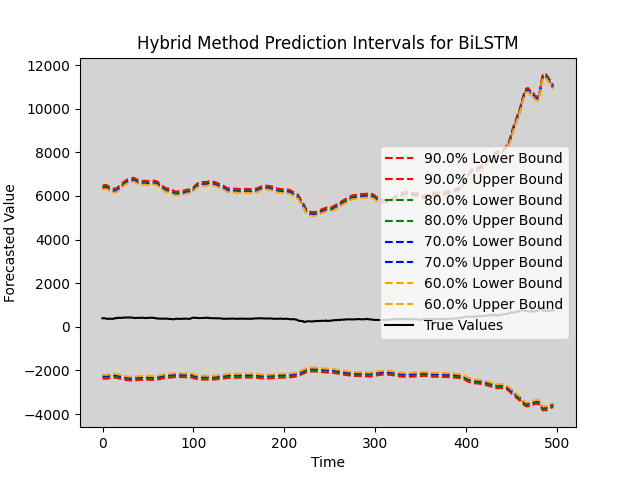
\includegraphics[width=\textwidth]{Chap03/figs/BiLSTM_hybrid_method_plot_AdaniPorts_Method2.png}
            \caption{BiLSTM.}
        \end{subfigure}
        \hfill
        \begin{subfigure}[b]{\textwidth}
            \centering
            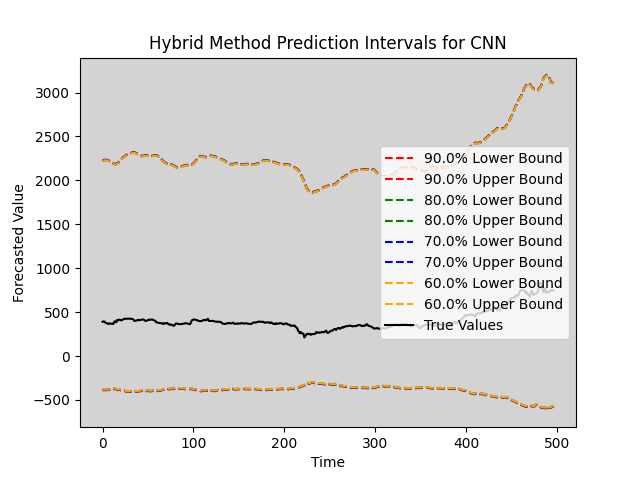
\includegraphics[width=\textwidth]{Chap03/figs/CNN_hybrid_method_plot_AdaniPorts_Method2.png}
            \caption{CNN.}
        \end{subfigure}
        \begin{subfigure}[b]{\textwidth}
            \centering
            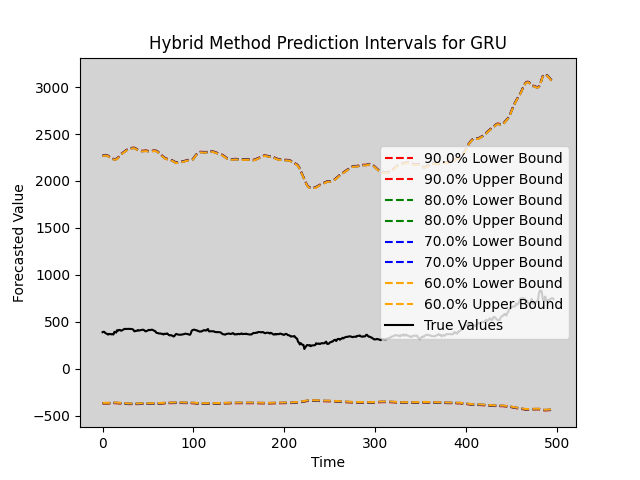
\includegraphics[width=\textwidth]{Chap03/figs/GRU_hybrid_method_plot_AdaniPorts_Method2.png}
            \caption{GRU.}
        \end{subfigure}
        \begin{subfigure}[b]{\textwidth}
            \centering
            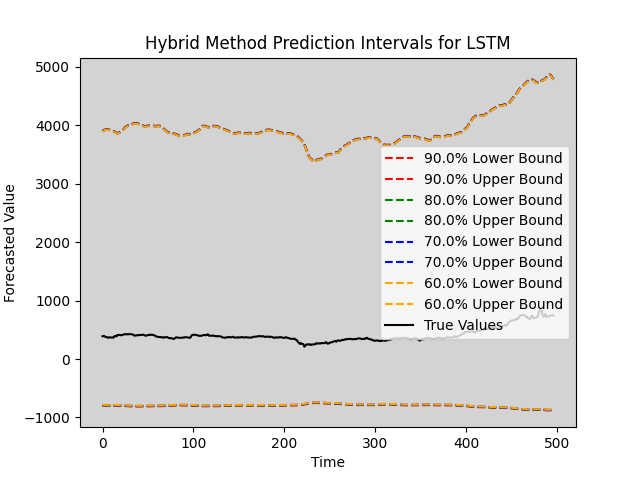
\includegraphics[width=\textwidth]{Chap03/figs/LSTM_hybrid_method_plot_AdaniPorts_Method2.png}
            \caption{LSTM.}
        \end{subfigure}
        \caption{Prediction Intervals for Adani Ports dataset obtained using proposed LUBE-Weibull based Hybrid Method and (a)BiLSTM, (b) CNN, (c) GRU, (d) LSTM Models.}
        \label{F 4.1}
    \end{minipage}
    \hfill
    \begin{minipage}{0.45\textwidth}
        \centering
        \begin{subfigure}[b]{\textwidth}
            \centering
            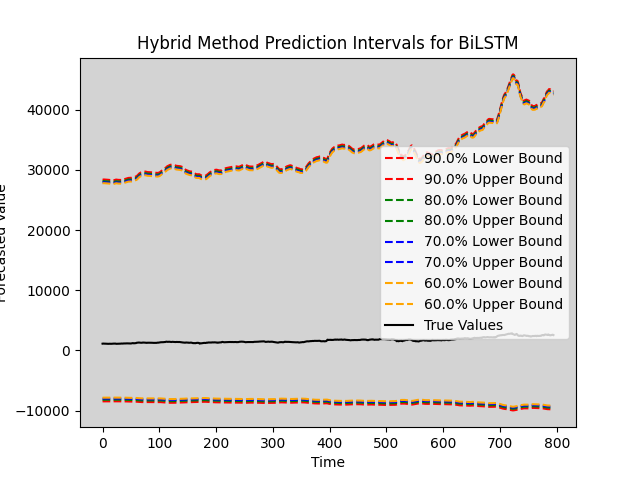
\includegraphics[width=\textwidth]{Chap03/figs/BiLSTM_hybrid_method_plot_AsianPaint_Method2.png}
            \caption{BiLSTM.}
        \end{subfigure}
        \hfill
        \begin{subfigure}[b]{\textwidth}
            \centering
            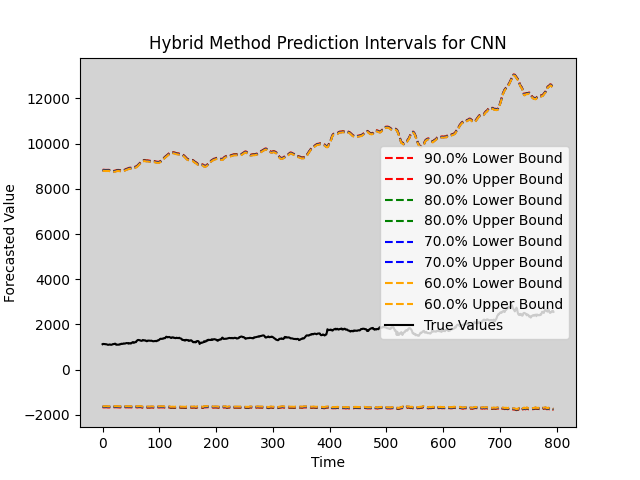
\includegraphics[width=\textwidth]{Chap03/figs/CNN_hybrid_method_plot_AsianPaint_Method2.png}
            \caption{CNN.}
        \end{subfigure}
        \begin{subfigure}[b]{\textwidth}
            \centering
            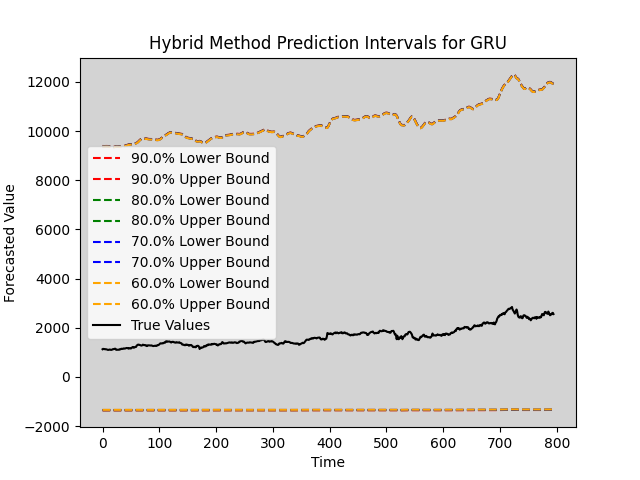
\includegraphics[width=\textwidth]{Chap03/figs/GRU_hybrid_method_plot_AsianPaint_Method2.png}
            \caption{GRU.}
        \end{subfigure}
        \begin{subfigure}[b]{\textwidth}
            \centering
            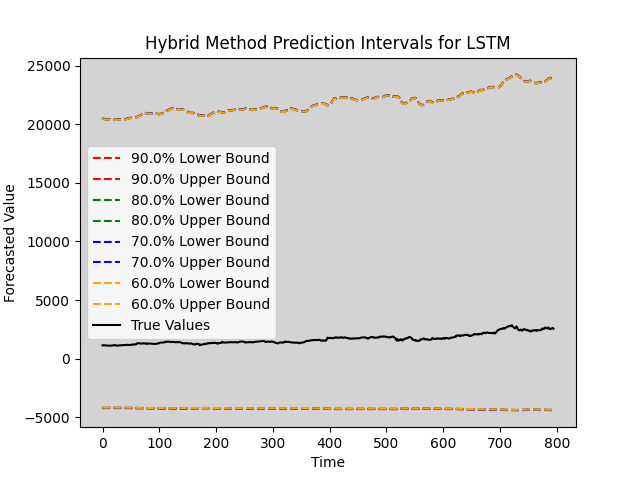
\includegraphics[width=\textwidth]{Chap03/figs/LSTM_hybrid_method_plot_AsianPaint_Method2.png}
            \caption{LSTM.}
        \end{subfigure}
        \caption{Prediction Intervals for Asian Paints dataset obtained using proposed LUBE-Weibull based Hybrid Method and (a)BiLSTM, (b) CNN, (c) GRU, (d) LSTM Models.}
        \label{F 4.2}
    \end{minipage}
\end{figure}


\begin{figure}[H]
    \centering
    \begin{minipage}{0.45\textwidth}
        \centering
        \begin{subfigure}[b]{\textwidth}
            \centering
            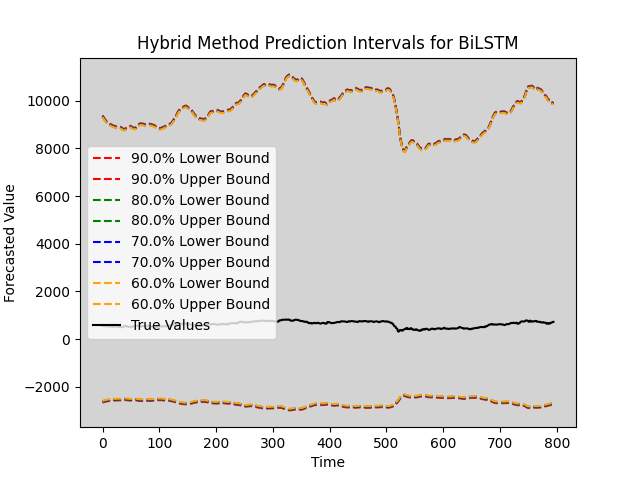
\includegraphics[width=\textwidth]{Chap03/figs/BiLSTM_hybrid_method_plot_AxisBank_Method2.png}
            \caption{BiLSTM.}
        \end{subfigure}
        \hfill
        \begin{subfigure}[b]{\textwidth}
            \centering
            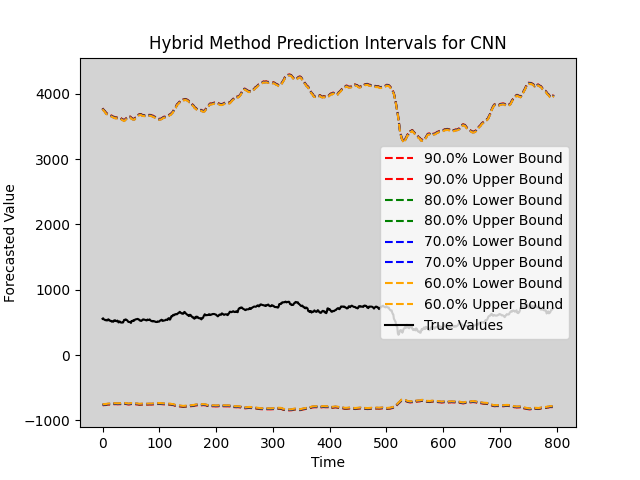
\includegraphics[width=\textwidth]{Chap03/figs/CNN_hybrid_method_plot_AxisBank_Method2.png}
            \caption{CNN.}
        \end{subfigure}
        \begin{subfigure}[b]{\textwidth}
            \centering
            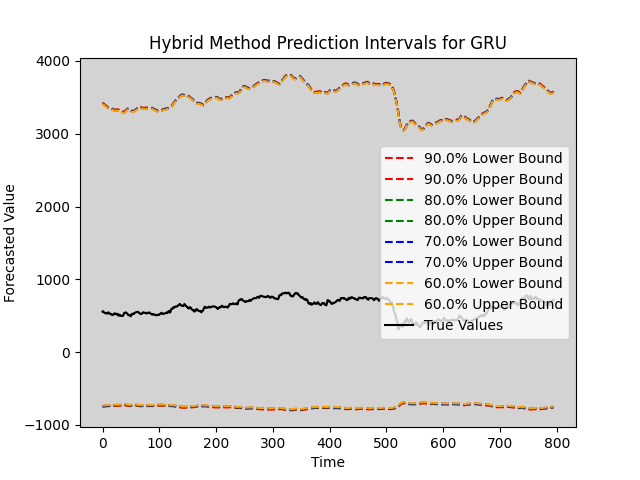
\includegraphics[width=\textwidth]{Chap03/figs/GRU_hybrid_method_plot_AxisBank_Method2.png}
            \caption{GRU.}
        \end{subfigure}
        \begin{subfigure}[b]{\textwidth}
            \centering
            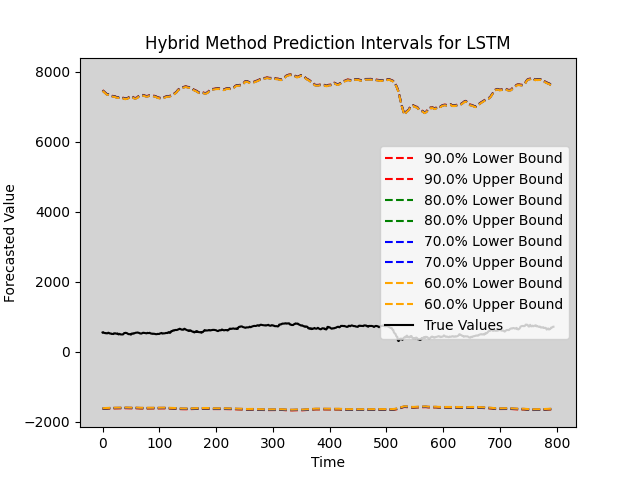
\includegraphics[width=\textwidth]{Chap03/figs/LSTM_hybrid_method_plot_AxisBank_Method2.png}
            \caption{LSTM.}
        \end{subfigure}
        \caption{Prediction Intervals for Axis Bank dataset obtained using proposed LUBE-Weibull based Hybrid Method and (a)BiLSTM, (b) CNN, (c) GRU, (d) LSTM Models.}
        \label{F 4.3}
    \end{minipage}
    \hfill
    \begin{minipage}{0.45\textwidth}
        \centering
        \begin{subfigure}[b]{\textwidth}
            \centering
            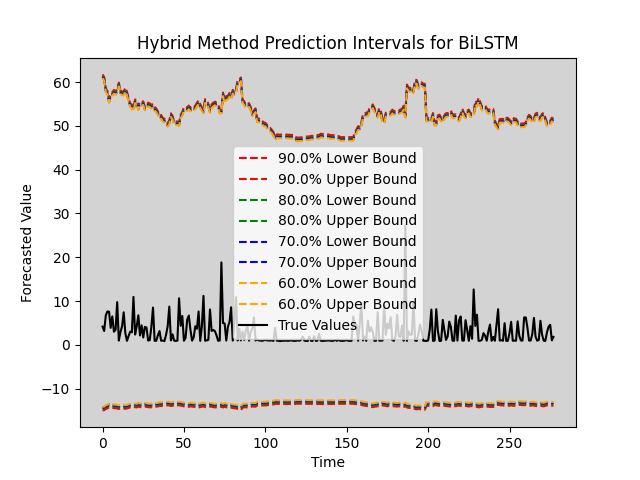
\includegraphics[width=\textwidth]{Chap03/figs/BiLSTM_hybrid_method_plot_Electricity_Consumption_Method2.png}
            \caption{BiLSTM.}
        \end{subfigure}
        \hfill
        \begin{subfigure}[b]{\textwidth}
            \centering
            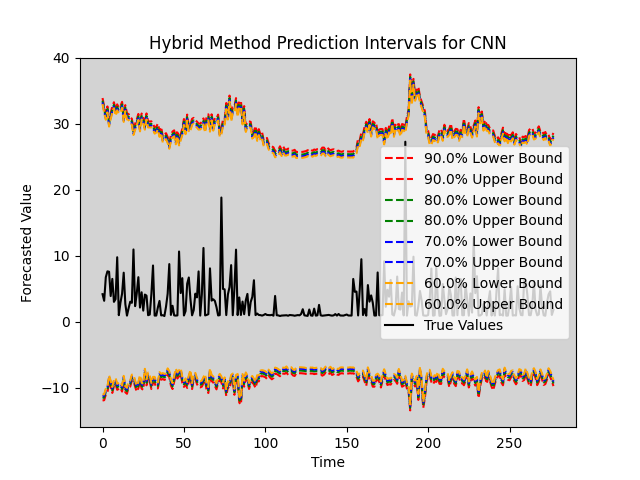
\includegraphics[width=\textwidth]{Chap03/figs/CNN_hybrid_method_plot_Electricity_Consumption_Method2.png}
            \caption{CNN.}
        \end{subfigure}
        \begin{subfigure}[b]{\textwidth}
            \centering
            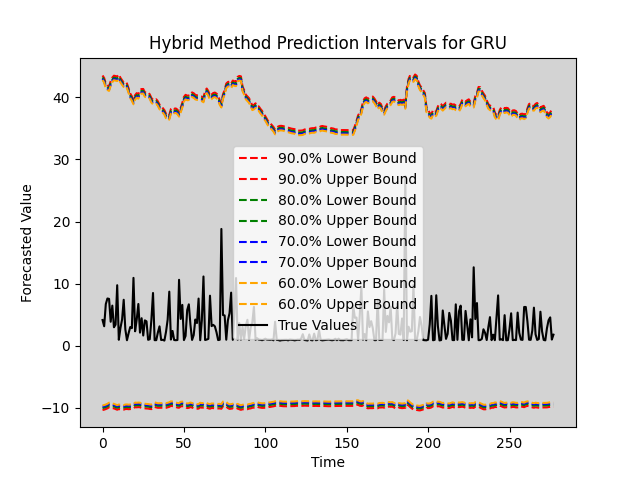
\includegraphics[width=\textwidth]{Chap03/figs/GRU_hybrid_method_plot_Electricity_Consumption_Method2.png}
            \caption{GRU.}
        \end{subfigure}
        \begin{subfigure}[b]{\textwidth}
            \centering
            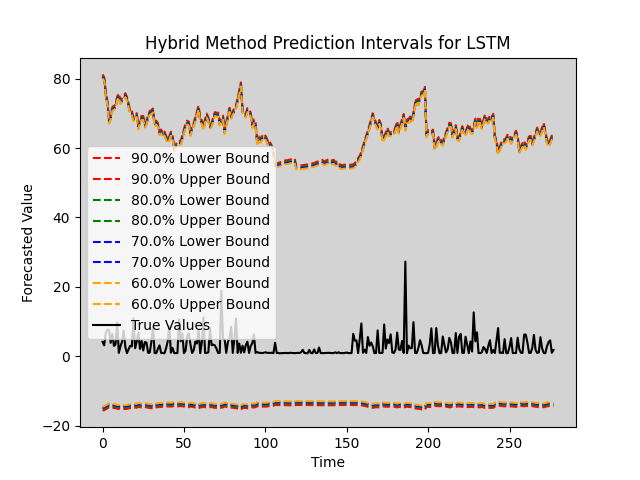
\includegraphics[width=\textwidth]{Chap03/figs/LSTM_hybrid_method_plot_Electricity_Consumption_Method2.png}
            \caption{LSTM.}
        \end{subfigure}
        \caption{Prediction Intervals for Electricity Consumption dataset obtained using proposed LUBE-Weibull based Hybrid Method and (a)BiLSTM, (b) CNN, (c) GRU, (d) LSTM Models.}
        \label{F 4.4}
    \end{minipage}
\end{figure}

\begin{figure}[H]
    \centering
        \begin{minipage}{0.4\textwidth}
            \centering
            \begin{subfigure}[b]{\textwidth}
                \centering
                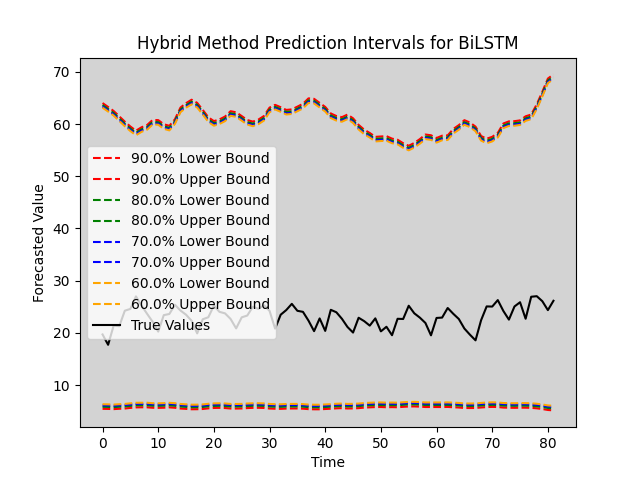
\includegraphics[width=\textwidth]{Chap03/figs/BiLSTM_hybrid_method_plot_Web_Traffic_Dataset_Method2.png}
                \caption{BiLSTM.}
            \end{subfigure}
            \hfill
            \begin{subfigure}[b]{\textwidth}
                \centering
                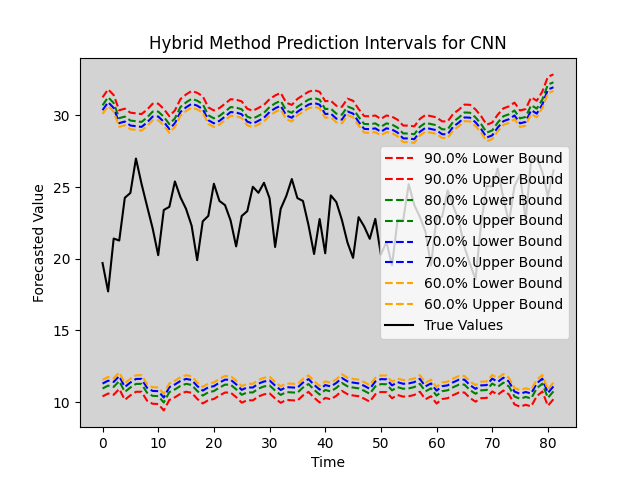
\includegraphics[width=\textwidth]{Chap03/figs/CNN_hybrid_method_plot_Web_Traffic_Dataset_Method2.png}
                \caption{CNN.}
            \end{subfigure}
            \begin{subfigure}[b]{\textwidth}
                \centering
                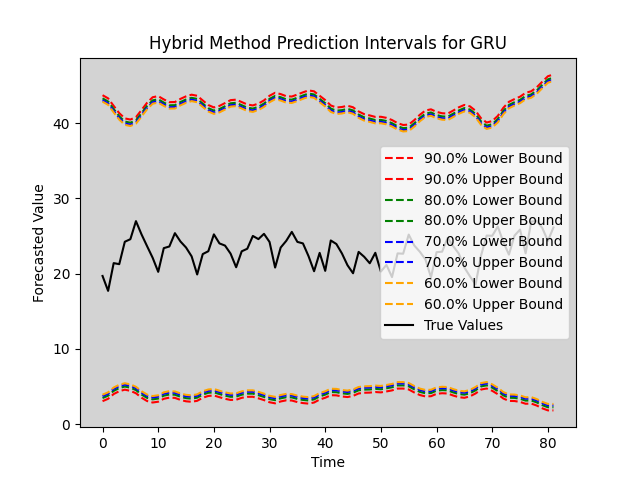
\includegraphics[width=\textwidth]{Chap03/figs/GRU_hybrid_method_plot_Web_Traffic_Dataset_Method2.png}
                \caption{GRU.}
            \end{subfigure}
            \begin{subfigure}[b]{\textwidth}
                \centering
                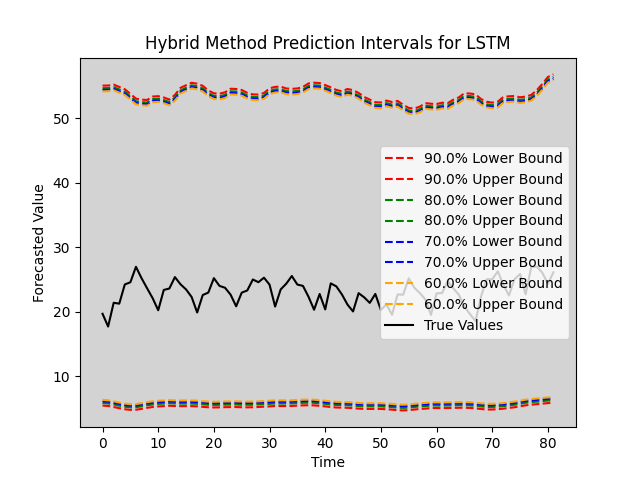
\includegraphics[width=\textwidth]{Chap03/figs/LSTM_hybrid_method_plot_Web_Traffic_Dataset_Method2.png}
                \caption{LSTM.}
            \end{subfigure}
        \end{minipage}
    
    \caption{Prediction Intervals for Web Traffic dataset obtained using proposed LUBE-Weibull based Hybrid Method and (a)BiLSTM, (b) CNN, (c) GRU, (d) LSTM Models.}
    \label{F 4.5}
\end{figure}

\begin{table*}[!t]
%\centering
\caption{Performance of LUBE-Weibull Hybrid Method on Adani Ports dataset.}
\vspace{0.5cm}
\renewcommand{\arraystretch}{1} % Adjust the value as needed
\resizebox{\textwidth}{!}{%
\begin{tabular}{|l|l|l|l|l|l|l|}
\hline
\textbf{Method Used} & \textbf{Confidence Level} & \textbf{Model} & \textbf{Avg PICP} & \textbf{Avg PINAW} &  \textbf{Avg ACE} & \textbf{Avg AWE} \\ \hline
\multirow{LUBE-Weibull Hybrid Method} 
& 0.6 & BiLSTM & 100 & 9.01 & 40 &  4995.50 \\ \cline{2-7}
& 0.6 & CNN & 100 & 4.15 & 40 & 1961.88 \\ \cline{2-7}
& 0.6 & GRU & 100 & 4.17 & 40 & 1979.80 \\ \cline{2-7}
& 0.6 & LSTM & 100 & 7.76 & 40 & 4218.70 \\ \cline{2-7}
& 0.7 & BiLSTM & 100 & 9.08 & 30 & 5039.80 \\ \cline{2-7}
& 0.7 & CNN & 100 & 4.16 & 30 & 1968.03 \\  \cline{2-7}
& 0.7 & GRU & 100 & 4.18 & 30 & 1984.13 \\ \cline{2-7}
& 0.7 & LSTM & 100 & 7.78 & 30 & 4227.40 \\ \cline{2-7}
& 0.8 & BiLSTM & 100 & 9.17 & 20 & 5093.81 \\ \cline{2-7}
& 0.8 & CNN & 100 & 4.17 & 20 & 1975.35 \\ \cline{2-7}
& 0.8 & GRU & 100 & 4.19 & 20 & 1989.29 \\ \cline{2-7}
& 0.8 & LSTM & 100 & 7.80 & 20 & 4237.76 \\ \cline{2-7}
& 0.9 & BiLSTM & 100 & 9.29 & 10 & 5170.50 \\ \cline{2-7}
& 0.9 & CNN & 100 & 4.18 & 10 & 1985.47 \\ \cline{2-7}
& 0.9 & GRU & 100 & 4.20 & 10 & 1996.40 \\ \cline{2-7}
& 0.9 & LSTM & 100 & 7.81 & 10 & 4252.00 \\ \hline
\end{tabular}%
}
\label{Table 3.1}
\end{table*}

\begin{table*}[!t]
%\centering
\caption{Performance of LUBE-Weibull Hybrid Method on Asian Paints dataset.}
\vspace{0.5cm}
\renewcommand{\arraystretch}{1} % Adjust the value as needed
\resizebox{\textwidth}{!}{%
\begin{tabular}{|l|l|l|l|l|l|l|}
\hline
\textbf{Method Used} & \textbf{Confidence Level} & \textbf{Model} & \textbf{Avg PICP} & \textbf{Avg PINAW} &  \textbf{Avg ACE} & \textbf{Avg AWE} \\ \hline
\multirow{LUBE-Weibull Hybrid Method} 
& 0.6 & BiLSTM & 100 & 23.37 & 40 & 39072.46 \\ \cline{2-7}
& 0.6 & CNN & 100 & 6.84 & 40 & 10198.06 \\ \cline{2-7}
& 0.6 & GRU & 100 & 7.41 & 40 & 11189.72 \\ \cline{2-7}
& 0.6 & LSTM & 100 & 15.27 & 40 & 24928.48 \\ \cline{2-7}
& 0.7 & BiLSTM & 100 & 23.56 & 30 & 39400.89 \\ \cline{2-7}
& 0.7 & CNN & 100 & 6.85 & 30 & 10219.74 \\ \cline{2-7}
& 0.7 & GRU & 100 & 7.42 & 30 & 11206.59 \\ \cline{2-7}
& 0.7 & LSTM & 100 & 15.28 & 30 & 24950.86 \\ \cline{2-7}
& 0.8 & BiLSTM & 100 & 23.78 & 20 & 39800.18 \\ \cline{2-7}
& 0.8 & CNN & 100 & 6.87 & 20 & 10245.51 \\ \cline{2-7}
& 0.8 & GRU & 100 & 7.43 & 20 & 11226.99 \\ \cline{2-7}
& 0.8 & LSTM & 100 & 15.30 & 20 & 24977.32 \\ \cline{2-7}
& 0.9 & BiLSTM & 100 & 24.11 & 10 & 40365.09 \\ \cline{2-7}
& 0.9 & CNN & 100 & 6.89 & 10 & 10280.97 \\ \cline{2-7}
& 0.9 & GRU & 100 & 7.44 & 10 & 11255.71 \\ \cline{2-7}
& 0.9 & LSTM & 100 & 15.32 & 10 & 25013.46 \\ \hline
\end{tabular}%
}
\label{Table 3.2}
\end{table*}

\begin{table*}[!t]
%\centering
\caption{Performance of LUBE-Weibull Hybrid Method on Axis Bank dataset.}
\vspace{0.5cm}
\renewcommand{\arraystretch}{1} % Adjust the value as needed
\resizebox{\textwidth}{!}{%
\begin{tabular}{|l|l|l|l|l|l|l|}
\hline
\textbf{Method Used} & \textbf{Confidence Level} & \textbf{Model} & \textbf{Avg PICP} & \textbf{Avg PINAW} &  \textbf{Avg ACE} & \textbf{Avg AWE} \\ \hline
\multirow{LUBE-Weibull Hybrid Method} 
& 0.6 & BiLSTM & 100 & 25.69 & 40 & 12517.84 \\ \cline{2-7}
& 0.6 & CNN & 100 & 8.70 & 40 & 3905.90 \\ \cline{2-7}
& 0.6 & GRU & 100 & 9.38 & 40 & 4250.76 \\ \cline{2-7}
& 0.6 & LSTM & 100 & 20.32 & 40 & 9793.09 \\ \cline{2-7}
& 0.7 & BiLSTM & 100 & 25.78 & 30 & 12562.57 \\ \cline{2-7}
& 0.7 & CNN & 100 & 8.72 & 30 & 3914.95 \\ \cline{2-7}
& 0.7 & GRU & 100 & 9.40 & 30 & 4259.08 \\ \cline{2-7}
& 0.7 & LSTM & 100 & 20.34 & 30 & 9805.74 \\ \cline{2-7}
& 0.8 & BiLSTM & 100 & 25.89 & 20 & 12616.01 \\ \cline{2-7}
& 0.8 & CNN & 100 & 8.74 & 20 & 3925.73 \\ \cline{2-7}
& 0.8 & GRU & 100 & 9.42 & 20 & 4269.04 \\ \cline{2-7}
& 0.8 & LSTM & 100 & 20.37 & 20 & 9820.72 \\ \cline{2-7}
& 0.9 & BiLSTM & 100 & 26.03 & 10 & 12689.96 \\ \cline{2-7}
& 0.9 & CNN & 100 & 8.77 & 10 & 3940.60 \\ \cline{2-7}
& 0.9 & GRU & 100 & 9.45 & 10 & 4282.84 \\ \cline{2-7}
& 0.9 & LSTM & 100 & 20.41 & 10 & 9841.23 \\ \hline

\end{tabular}%
}
\label{Table 3.3}
\end{table*}

\begin{table*}[!t]
%\centering
\caption{Performance of LUBE-Weibull Hybrid Method on Electricity Consumption dataset.}
\vspace{0.5cm}
\renewcommand{\arraystretch}{1} % Adjust the value as needed
\resizebox{\textwidth}{!}{%
\begin{tabular}{|l|l|l|l|l|l|l|}
\hline
\textbf{Method Used} & \textbf{Confidence Level} & \textbf{Model} & \textbf{Avg PICP} & \textbf{Avg PINAW} &  \textbf{Avg ACE} & \textbf{Avg AWE} \\ \hline
\multirow{LUBE-Weibull Hybrid Method} 
& 0.6 & BiLSTM & 100 & 2.54 & 40 & 40.62 \\ \cline{2-7}
& 0.6 & CNN & 100 & 1.37 & 40 & 9.85 \\ \cline{2-7}
& 0.6 & GRU & 100 & 1.86 & 40 & 22.64 \\ \cline{2-7}
& 0.6 & LSTM & 100 & 2.84 & 40 & 48.53 \\ \cline{2-7}
& 0.7 & BiLSTM & 100 & 2.55 & 30 & 41.07 \\ \cline{2-7}
& 0.7 & CNN & 100 & 1.39 & 30 & 10.30 \\ \cline{2-7}
& 0.7 & GRU & 100 & 1.87 & 30 & 23.01 \\ \cline{2-7}
& 0.7 & LSTM & 100 & 2.86 & 30 & 49.06 \\ \cline{2-7}
& 0.8 & BiLSTM & 100 & 2.57 & 20 & 41.60 \\ \cline{2-7}
& 0.8 & CNN & 100 & 1.41 & 20 & 10.85 \\ \cline{2-7}
& 0.8 & GRU & 100 & 1.89 & 20 & 23.46 \\ \cline{2-7}
& 0.8 & LSTM & 100 & 2.88 & 20 & 49.71 \\ \cline{2-7}
& 0.9 & BiLSTM & 100 & 2.60 & 10 & 42.35 \\ \cline{2-7}
& 0.9 & CNN & 100 & 1.44 & 10 & 11.65 \\ \cline{2-7}
& 0.9 & GRU & 100 & 1.91 & 10 & 24.10 \\ \cline{2-7}
& 0.9 & LSTM & 100 & 2.91 & 10 & 50.61 \\ \hline
\end{tabular}%
}
\label{Table 3.4}
\end{table*}

\begin{table*}[!t]
%\centering
\caption{Performance of LUBE-Weibull Hybrid Method on Web Traffic dataset.}
\vspace{0.5cm}
\renewcommand{\arraystretch}{1} % Adjust the value as needed
\resizebox{\textwidth}{!}{%
\begin{tabular}{|l|l|l|l|l|l|l|}
\hline
\textbf{Method Used} & \textbf{Confidence Level} & \textbf{Model} & \textbf{Avg PICP} & \textbf{Avg PINAW} &  \textbf{Avg ACE} & \textbf{Avg AWE} \\ \hline
\multirow{LUBE-Weibull Hybrid Method} 
& 0.6 & BiLSTM & 100 & 6.04 & 40 & 46.91 \\ \cline{2-7}
& 0.6 & CNN & 100 & 2.16 & 40 & 10.82 \\ \cline{2-7}
& 0.6 & GRU & 100 & 3.65 & 40 & 24.64 \\ \cline{2-7}
& 0.6 & LSTM & 100 & 5.35 & 40 & 40.52 \\ \cline{2-7}
& 0.7 & BiLSTM & 100 & 6.09 & 30 & 47.37 \\ \cline{2-7}
& 0.7 & CNN & 100 & 2.21 & 30 & 11.27 \\ \cline{2-7}
& 0.7 & GRU & 100 & 3.70 & 30 & 25.11 \\ \cline{2-7}
& 0.7 & LSTM & 100 & 5.40 & 30 & 40.96 \\ \cline{2-7}
& 0.8 & BiLSTM & 100 & 6.15 & 20 & 47.94 \\ \cline{2-7}
& 0.8 & CNN & 100 & 2.27 & 20 & 11.86 \\ \cline{2-7}
& 0.8 & GRU & 100 & 3.76 & 20 & 25.73 \\ \cline{2-7}
& 0.8 & LSTM & 100 & 5.46 & 20 & 41.52 \\ \cline{2-7}
& 0.9 & BiLSTM & 100 & 6.24 & 10 & 48.76 \\ \cline{2-7}
& 0.9 & CNN & 100 & 2.37 & 10 & 12.79 \\ \cline{2-7}
& 0.9 & GRU & 100 & 3.87 & 10 & 26.69 \\ \cline{2-7}
& 0.9 & LSTM & 100 & 5.55 & 10 & 42.35 \\ \hline
\end{tabular}%
}
\label{Table 3.5}
\end{table*}
\clearpage

\subsection{Discussion}
The results demonstrate that the LUBE-Weibull Hybrid Method maintains 100\% PICP like the standalone LUBE method without compromising acceptable PINAW values. The ACE values reflect that the method achieves confidence levels that are essentially similar to the target measures. Additionally, the AWE values confirms that the Weibull-based adjustment prevents the over-broadening of prediction intervals.
We have certainly achieved better results than the traditional LUBE method while also significantly reducing the required time and computational requirements by incorporating the Weibull method.

The last section provides a summary of the research and suggests potential avenues for future research.

\section{Summary}
This chapter introduced the LUBE-Weibull Based Hybrid Approach to probabilistic time series forecasting, which integrates deep learning-driven prediction interval estimation with Weibull-based residual correction. Experimental results demonstrate that the hybrid approach outperforms the Traditional LUBE Method in terms of improving coverage probability (PICP) with an acceptable balance between interval sharpness (PINAW) and accuracy (ACE). Deployment of Weibull-based correction effectively sharpens prediction intervals by accounting for residual uncertainties, thus improving forecast reliability.

Comparison with the Advanced LUBE Method reveals that the hybrid approach has a marginally increased AWE, indicating slightly wider prediction intervals. However, this feature may offer a potential benefit: the Hybrid Method is computationally more efficient, as it removes extra complexity in the loss function while performing post-hoc corrections to sharpen interval estimation. This trade-off suggests that the Hybrid Method offers a viable and scalable alternative to Advanced LUBE, especially in situations requiring tradeoff between computational cost and forecasting quality.

Future research can explore adaptive scaling of Weibull corrections to further improve interval sharpness without compromising coverage. Moreover, the use of uncertainty-aware deep learning architectures or ensembling of heterogeneous architectures may potentially improve predictive quality.

\chapter{LUBE-QR Based Hybrid Method For Probabilistic Time Series Forecasting}\label{January Update}

\section{ Motivation}
Forecasting is very important in domains like energy, finance, healthcare, and climatology, as accurate predictions allow for well-informed and efficient decision making. While traditional forecasting methodologies tend to produce point estimates, they have the disadvantage of excluding uncertainty, an oversight that can lead to erroneous conclusions and inefficient use of resources, especially in risky scenarios. Probabilistic forecasting rectifies this by providing prediction intervals (PIs) that estimate uncertainty and allow for risk informed decision making. However, choice of the most appropriate method is a major problem. Parametric methods, including Gaussian and Weibull Distribution based methods, are computationally efficient but can fall short of capturing complex patterns in the data. Non-parametric methods, like Quantile Regression and Bootstrap-based methods are more data adaptive and versatile but are computationally demanding.

The Lower Upper Bound Estimation (LUBE) algorithm, a deep learning-based non-parametric algorithm, learns PIs from data but lacks reliability in highly dynamic environments. 
Weibull distribution modeling, in contrast, models residual errors accurately but lacks adaptability to time-dependent forecast changes.

This chapter presents the LUBE-QR Based Hybrid Method, a technique that improves PI reliability through the combination of deep learning-based LUBE prediction and QR-based residual correction. 

The technique consists of using deep learning models (LSTM, CNN, GRU, BiLSTM) to produce initial prediction intervals, and residual error modeling through QR method.
The QR-based corrections improve the intervals, which improves accuracy and stability at various confidence levels. 

Through the combination of the flexibility of deep learning and statistical error modeling, the technique presents stronger and more reliable probabilistic predictions. 


\section{Methodology}
\subsection{Data Pre-processing}
The time series datasets are preprocessed to ensure stable training and effective modeling. First, the data is normalized to the range [0,1] using MinMaxScaler. Next, a sliding window approach with a window size of 12 is applied to generate input-output pairs, where the past 12 time steps are used to predict the next step. Finally, the dataset is divided into three subsets: 70\% for training, 15\% for validation, and 15\% for testing, ensuring a balanced and robust evaluation of the model.

\subsection{Model Selection}
The hybrid method employs different deep learning architectures to generate first-stage prediction intervals (PIs). Long Short-Term Memory (LSTM) is well suited to learning long-term dependencies of sequential data, while Convolutional Neural Networks (CNN) are best at detecting local patterns and trends. Gated Recurrent Units (GRU) offer a computationally cheaper option that still retains the ability to learn sequences. Additionally, Bidirectional LSTM (BiLSTM) enhances feature extraction through learning information in both directions. Each model delivers two outputs for each prediction, which represent the lower and upper bounds of the PI and hence enable extensive estimation of uncertainty.

\subsection{LUBE Loss Function}
The LUBE method directly learns interval bounds using a custom loss function. The LUBE loss function is defined as:

\begin{equation}
\mathcal{L}_{\text{LUBE}} = \text{PINAW} + \lambda \cdot \max\left(0,\left(1 - \text{PICP}_{\text{target}}\right) - \text{PICP} \right)^2
\label{LUBE Loss Function}
\end{equation}

Where:
\begin{itemize}
    \item PINAW is Prediction Interval Normalized Average Width, which penalizes wide intervals.
    
    \item PICP is Prediction Interval Coverage Probability, representing the fraction of true values that lie within the predicted intervals.
    
    \item $\lambda$ is a regularization hyperparameter that controls the trade-off between narrow intervals and sufficient coverage.
    
    \item $UB_i$, $LB_i$ are the predicted upper and lower bounds for the $i^{\text{th}}$ data point.
    
    \item $y_i$ is the true value of the $i^{\text{th}}$ sample.
    
    \item $\text{PICP}_{\text{target}}$ is the desired confidence level, such as 0.9, 0.8, 0.7 or 0.6.
    
    \item R is the range of the training target values, used to normalize the interval width.
    
    \item $\mathbb{I}(\cdot)$ is the indicator function, which returns 1 if the condition inside is true, and 0 otherwise.
\end{itemize}

The loss aims to produce prediction intervals that are as narrow as possible (minimizing $\text{PINAW}$), while ensuring they capture the true target values with the desired coverage level (maximizing $\text{PICP}$).

\\

\subsection{QR-Based Residual Correction}

After generating initial prediction intervals $[LB_i, UB_i]$ using the Advanced LUBE method, the Hybrid LUBE–QR framework applies a correction based on quantile regression to refine the interval bounds using residual information.

Let the residuals be defined as:
\begin{equation}
r_i = |y_i - \hat{y}_i|
\label{residual}
\end{equation}
where $y_i$ is the true target value and $\hat{y}_i = \frac{LB_i + UB_i}{2}$ is the midpoint (mean prediction) of the LUBE interval.

A Quantile Regression (QR) model is then trained to estimate specific conditional quantiles of the residuals, denoted as $Q_{\tau}(r|x)$, where $\tau$ represents the desired quantile level (e.g., $\tau = 0.9, 0.95$). The model learns to predict asymmetric quantiles based on the input features $x$.

For a target confidence level $c$, we determine the corresponding quantile correction $\delta_c$ such that:
\begin{equation}
\delta_c = Q_{1 - \frac{1 - c}{2}}(r|x)
\label{quantile correction}
\end{equation}

The final corrected prediction interval is:
\begin{subequations} \label{eq:corrected_bounds}
\begin{align}
LB_i^{\text{corrected}} &= \hat{y}_i - \delta_c \\
UB_i^{\text{corrected}} &= \hat{y}_i + \delta_c
\end{align}
\end{subequations}


The Eq. \ref{quantile correction} shows the quantile correction formula while the Eq. \ref{eq:corrected_bounds} shows the corrected Lower Bound and Upper Bound obtained. This residual-based QR correction enables the prediction intervals to better account for heteroscedasticity and non-Gaussian uncertainty structures, resulting in intervals that are not only statistically valid but also adaptive to local data variability.
\\

\subsection{Confidence Levels and Performance Metrics}
The hybrid method examines prediction intervals for four confidence levels: 90\%, 80\%, 70\%, and 60\%, giving a complete uncertainty estimation evaluation. Performance is measured via several key indicators. Prediction Interval Coverage Probability (PICP) estimates the percentage of actual values in the predicted interval, assessing reliability. Prediction Interval Normalized Average Width (PINAW) estimates interval sharpness as a function of data range, sacrificing precision for coverage. Average Coverage Error (ACE) estimates PICP deviation from the target confidence level, measuring calibration accuracy. Lastly, Average Width Error (AWE) evaluates how far interval width is from expected bounds, ensuring proper uncertainty quantification.

\subsection{Probabilistic Forecasting using Hybrid LUBE-QR Based Method}
\begin{algorithm}
    \small
    %\normalsize
    \SetAlgoNlRelativeSize{0}
    \SetAlgoCaptionSeparator{:}
    
    \KwIn{Time series dataset $D$}
    \KwOut{Predicted intervals $[LB', UB']$, PICP, PINAW, ACE, AWE}
    
    \textbf{Step 1: Data Preprocessing}\\
    Normalize $D$ using MinMaxScaler\\
    Generate input-output pairs with window size $w$\\
    Split into train, validation, and test sets\\
    
    \textbf{Step 2: Define Advanced LUBE Loss}\\
    \ForEach{$c \in \{0.9, 0.8, 0.7, 0.6\}$}{
        $q = 1 - c$\\
        Compute $LB$, $UB$\\
        Compute $\text{Loss}_{\text{lower}}$\\
        Compute $\text{Loss}_{\text{upper}}$\\
        Compute PICP (as in Eq.~\eqref{Equation 1}) and PINAW (as in Eq.~\eqref{Equation 2})\\
        Compute $\text{Loss}_{\text{LUBE}}$ (as in Eq.~\eqref{LUBE Loss Function}).
    }
    
    \textbf{Step 3: Model Training}\\
    \ForEach{$M \in \{$LSTM, CNN, GRU, BiLSTM$\}$}{
        Define model architecture\\
        Compile with Advanced LUBE loss\\
        Train on $(X_{\text{train}}, y_{\text{train}})$ for $e$ epochs\\
        Validate on $(X_{\text{val}}, y_{\text{val}})$\\
        Predict LUBE bounds $LB, UB$ on test data\\
        Compute midpoint $\hat{y}$
    }
    
    \textbf{Step 4: Fit Quantile Regression on Residuals}\\
    Compute residuals (as in Eq. \eqref{residual})\\
    \ForEach{$c \in \{0.9, 0.8, 0.7, 0.6\}$}{
        Train Quantile Regression models to estimate:\\
        Lower quantile and Upper quantile\\
        Predict residual quantiles $\hat{r}_{\text{lower}}, \hat{r}_{\text{upper}}$\\
    }
    
    \textbf{Step 5: Adjust Prediction Intervals Using QR Correction}\\
    \ForEach{$c \in \{0.9, 0.8, 0.7, 0.6\}$}{
        $LB' = \hat{y} + \hat{r}_{\text{lower}}$\\
        $UB' = \hat{y} + \hat{r}_{\text{upper}}$\\
    }

    \textbf{Step 6: Evaluation Metrics} Compute the PICP (as in Eq.~\eqref{Equation 1}), PINAW (as in Eq. ~\eqref{Equation 2}), ACE (as in Eq. ~\eqref{Equation 3}) and AWE (as in Eq. ~\eqref{Equation 4}) of the computed prediction intervals.

    
    \textbf{Step 7: Aggregate Results}\\
    \text{Compute mean of metrics for each case}\\
    
    \caption{Hybrid LUBE–QR Method.}
\end{algorithm}

The crux of this algorithm begins with training deep-learning models (LSTM, BiLSTM, CNN, GRU) on a tailored LUBE loss function that is specifically tailored to optimize interval width and violation of coverage. For each pre-specified confidence level (0.6, 0.7, 0.8, 0.9), the LUBE loss is dynamically scaled to penalize the failure of prediction intervals to cover the true values. This training produces initial lower and upper bounds for the target variable, which are the initial prediction intervals.

Lastly, the method estimates the midpoint of the LUBE-generated intervals and the absolute residuals between the predicted midpoint and observed target values are estimated. These residuals are the systematic forecasting errors not explained by the original model. Quantile Regression is applied to the residuals to estimate the lower and upper quantiles at each confidence level. This helps to model the residual distribution in a non-parametric and data-adaptive manner. The quantile forecasts are subsequently combined with the forecasted midpoint to provide improved lower and upper limits for the final prediction intervals. The two-stage adjustment process enables the model to improve its interval estimates by exploiting both interval-targeted loss optimization and quantile-based residual learning.

For each run and model, the following metrics are computed for each run and model to measure the quality of the prediction intervals: Prediction Interval Coverage Probability (PICP), Prediction Interval Normalized Average Width (PINAW), Average Coverage Error (ACE) and Absolute Width Error (AWE). The whole process is repeated for 10 independent runs for all types of models and confidence levels to provide statistical robustness. Finally, the results are aggregated and saved in structured CSV formats, and graphical visualizations are generated for all models, showing the predicted intervals over the test data for different confidence levels.

%\newpage
\section{Results and Discussions}
This section displays the evaluation of the LUBE-QR Based Hybrid Method across five datasets. The performance of the hybrid approach is assessed using metrics PICP, PINAW, ACE and AWE. The results are visualized through prediction interval plots and summarized in tables.\\ 

Figures \ref{fig 5.1}, \ref{fig 5.2}, \ref{fig 5.3}, \ref{fig 5.4} and \ref{fig 5.5} shows Prediction Intervals for all the five different datasets obtained using proposed LUBE-QR based Hybrid Method and (a) BiLSTM, (b) CNN, (c) GRU, (d) LSTM Models respectively.\\

Tables \ref{table 5.1}, \ref{table 5.2}, \ref{table 5.3}, \ref{table 5.4} and \ref{table 5.5} shows the performance of the proposed LUBE-QR based Hybrid Method on all the five datasets respectively across the four metrics PICP, PINAW, ACE and AWE for four different confidence levels 60\%, 70\%, 80\% and 90\%.\\

It is visible from Figures \ref{fig 5.1} to \ref{fig 5.5} and from Tables \ref{table 5.1} to \ref{table 5.5} that the results obtained from this Hybrid LUBE-QR method produces crisp and sharp intervals while maintaining low values of PINAW, ACE and AWE. This makes this hybrid model a good alternative to existing traditional models for real time probabilistic forecasting tasks.

\subsection{Visualization Of Prediction Intervals}

\begin{figure}[H]
    \centering
    \begin{minipage}{0.49\textwidth}
        \centering
        \begin{subfigure}[b]{\textwidth}
            \centering
            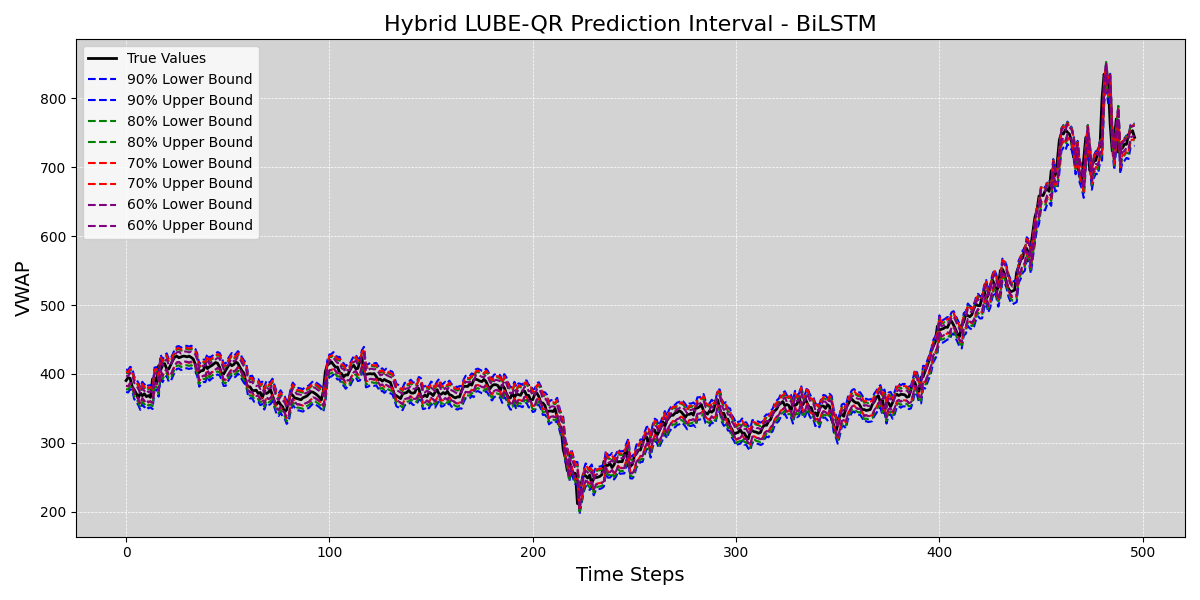
\includegraphics[width=\textwidth]{Chap03/figs/AP_Hybrid_LUBE_QR_AllConfidence_BiLSTM.png}
            \caption{BiLSTM.}
        \end{subfigure}
        \hfill
        \begin{subfigure}[b]{\textwidth}
            \centering
            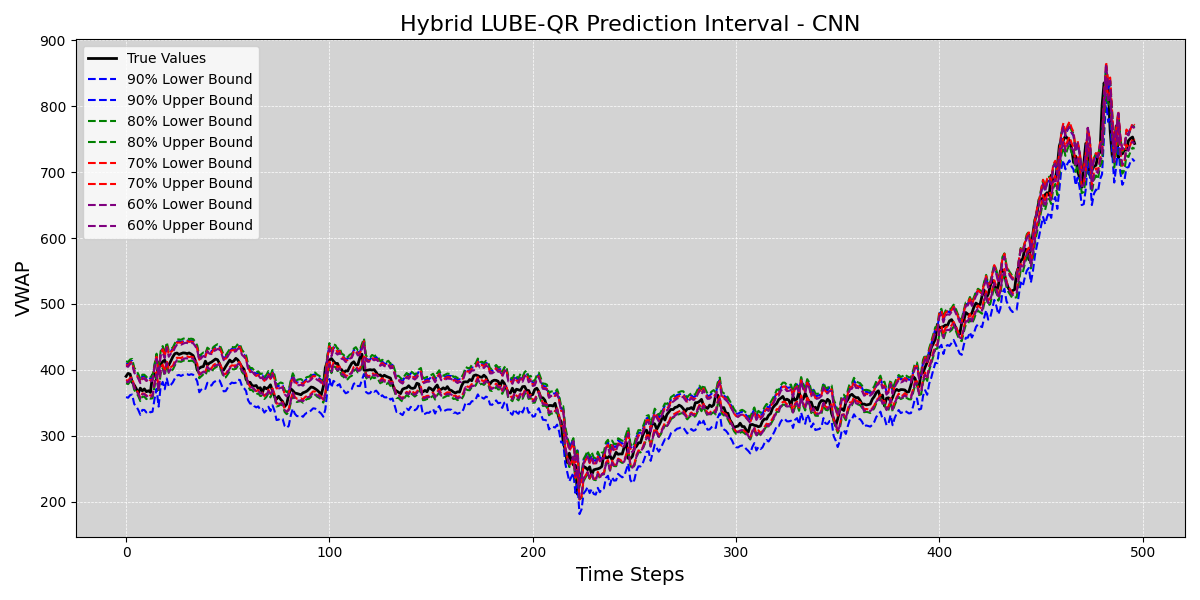
\includegraphics[width=\textwidth]{Chap03/figs/AP_Hybrid_LUBE_QR_AllConfidence_CNN.png}
            \caption{CNN.}
        \end{subfigure}
        \begin{subfigure}[b]{\textwidth}
            \centering
            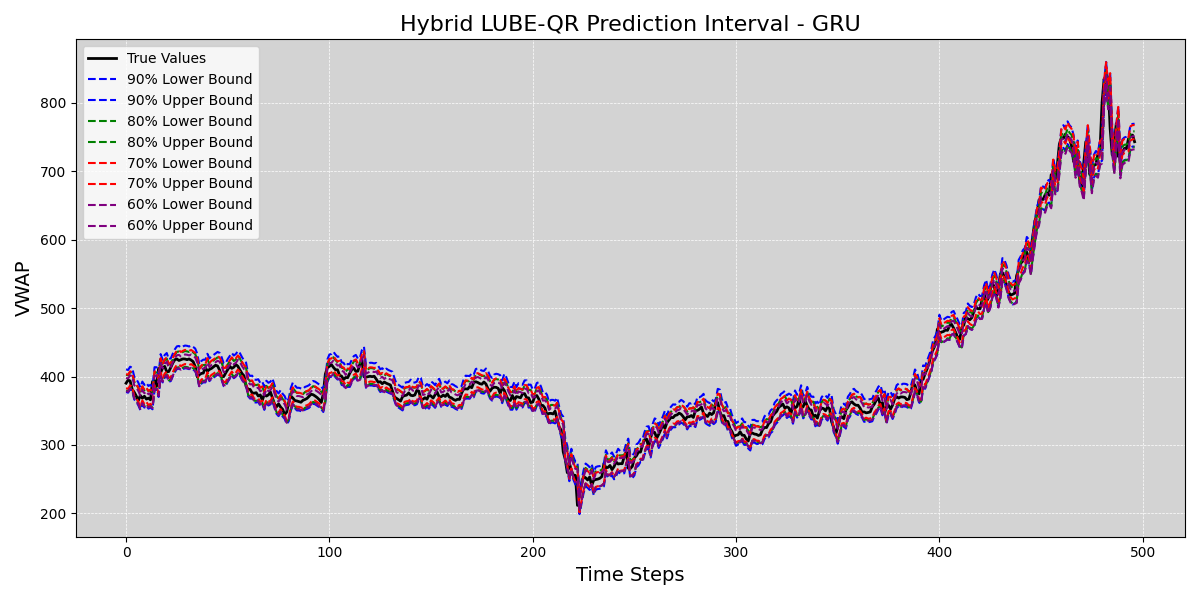
\includegraphics[width=\textwidth]{Chap03/figs/AP_Hybrid_LUBE_QR_AllConfidence_GRU.png}
            \caption{GRU.}
        \end{subfigure}
        \begin{subfigure}[b]{\textwidth}
            \centering
            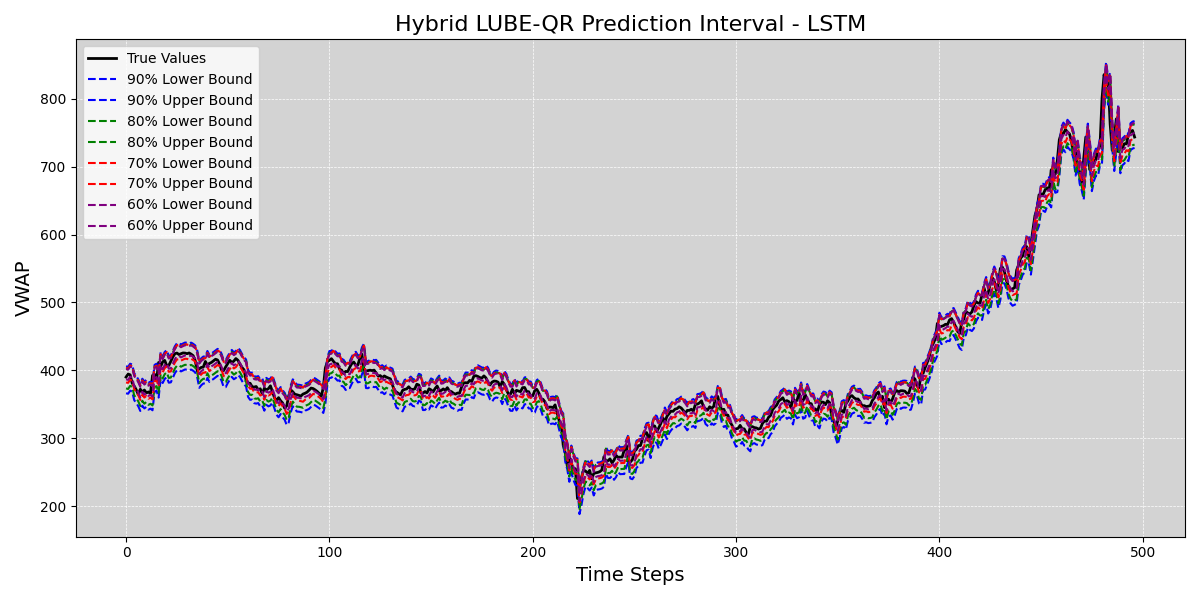
\includegraphics[width=\textwidth]{Chap03/figs/AP_Hybrid_LUBE_QR_AllConfidence_LSTM.png}
            \caption{LSTM.}
        \end{subfigure}
        \caption{Prediction Intervals for Adani Ports dataset obtained using proposed LUBE-QR based Hybrid Method and (a) BiLSTM, (b) CNN, (c) GRU, (d) LSTM Models respectively.}
        \label{fig 5.1}
    \end{minipage}
    \hfill
    \begin{minipage}{0.49\textwidth}
        \centering
        \begin{subfigure}[b]{\textwidth}
            \centering
            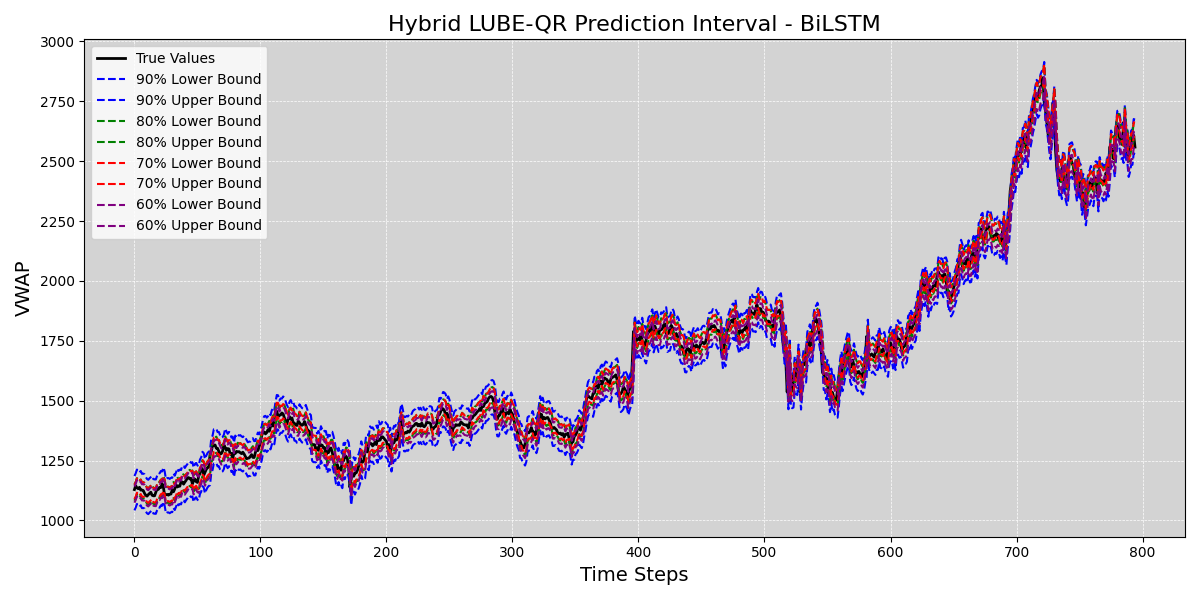
\includegraphics[width=\textwidth]{Chap03/figs/AsianPaint_Hybrid_LUBE_QR_AllConfidence_BiLSTM.png}
            \caption{BiLSTM.}
        \end{subfigure}
        \hfill
        \begin{subfigure}[b]{\textwidth}
            \centering
            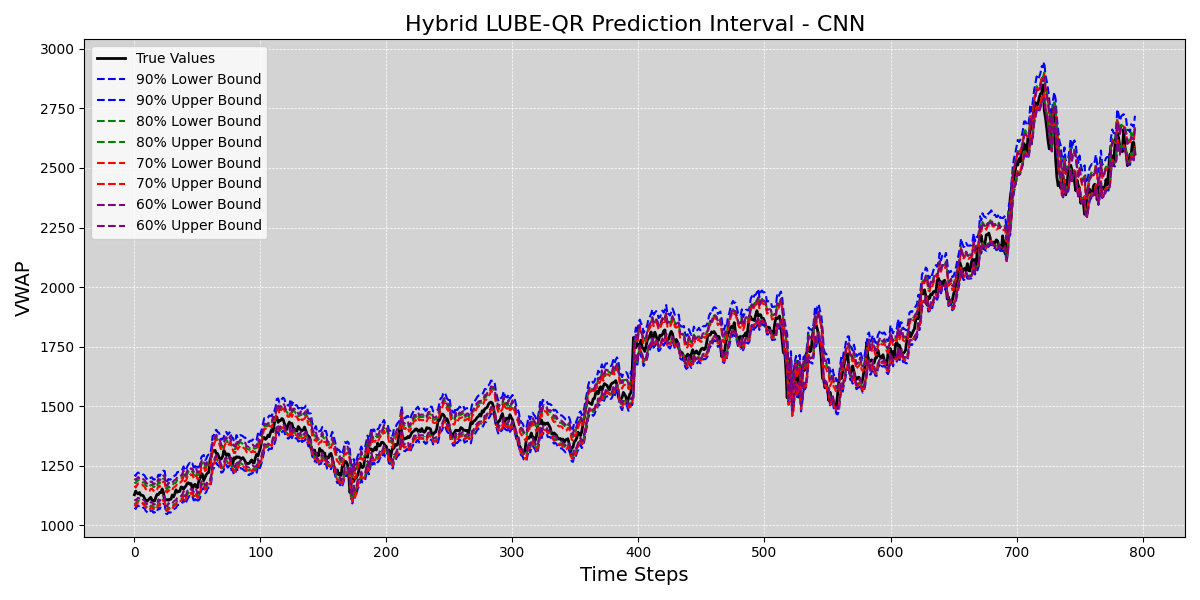
\includegraphics[width=\textwidth]{Chap03/figs/AsianPaint_Hybrid_LUBE_QR_AllConfidence_CNN.png}
            \caption{CNN.}
        \end{subfigure}
        \begin{subfigure}[b]{\textwidth}
            \centering
            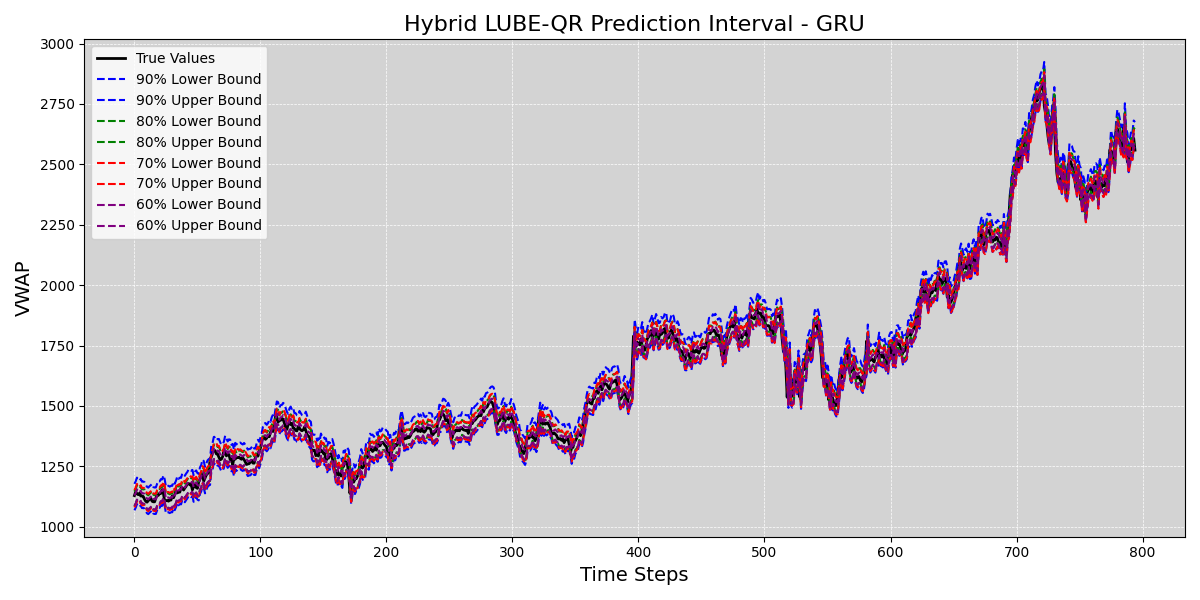
\includegraphics[width=\textwidth]{Chap03/figs/AsianPaint_Hybrid_LUBE_QR_AllConfidence_GRU.png}
            \caption{GRU.}
        \end{subfigure}
        \begin{subfigure}[b]{\textwidth}
            \centering
            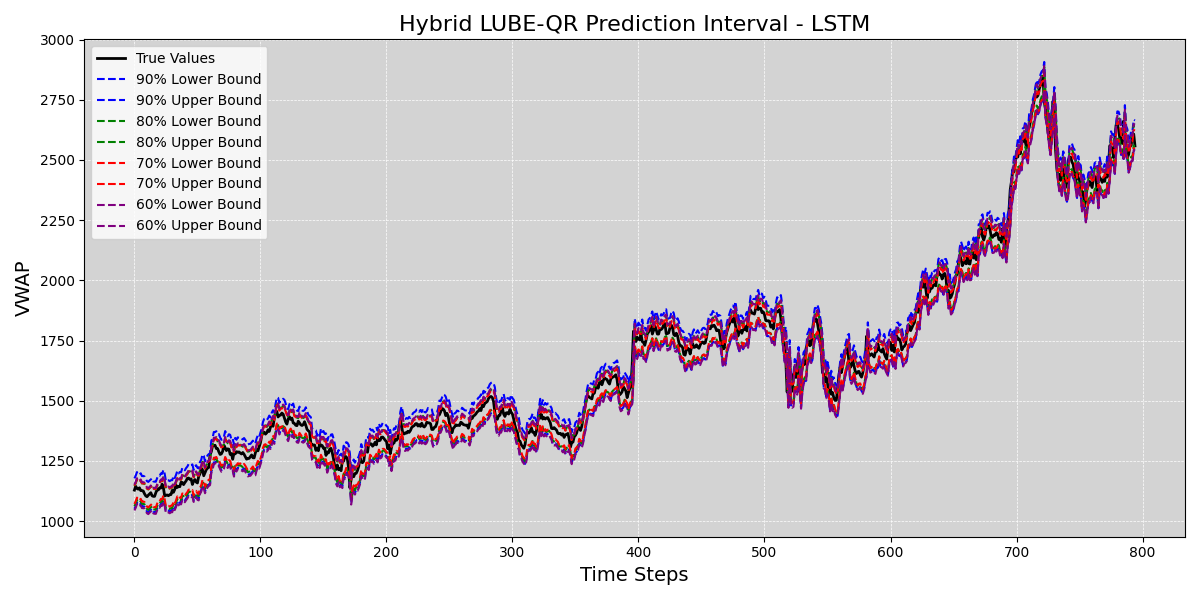
\includegraphics[width=\textwidth]{Chap03/figs/AsianPaint_Hybrid_LUBE_QR_AllConfidence_LSTM.png}
            \caption{LSTM.}
        \end{subfigure}
        \caption{Prediction Intervals for Asian Paints dataset obtained using proposed LUBE-QR based Hybrid Method and (a) BiLSTM, (b) CNN, (c) GRU, (d) LSTM Models respectively.}
        \label{fig 5.2}
    \end{minipage}
\end{figure}


\begin{figure}[H]
    \centering
    \begin{minipage}{0.49\textwidth}
        \centering
        \begin{subfigure}[b]{\textwidth}
            \centering
            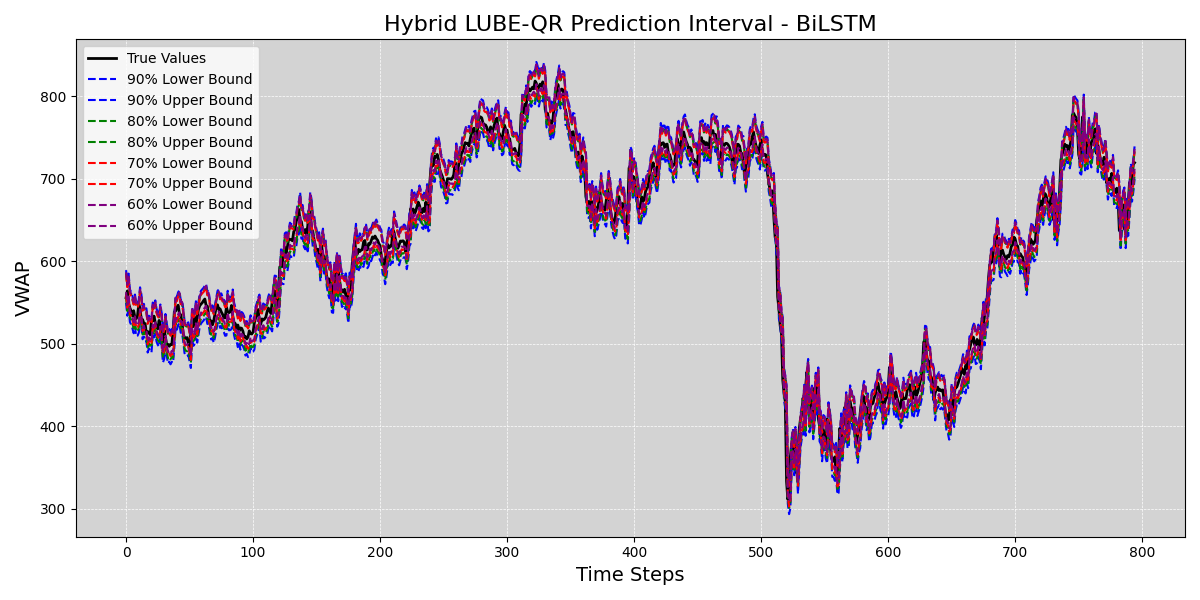
\includegraphics[width=\textwidth]{Chap03/figs/Hybrid_LUBE_QR_AllConfidence_axisbank_BiLSTM.png}
            \caption{BiLSTM.}
        \end{subfigure}
        \hfill
        \begin{subfigure}[b]{\textwidth}
            \centering
            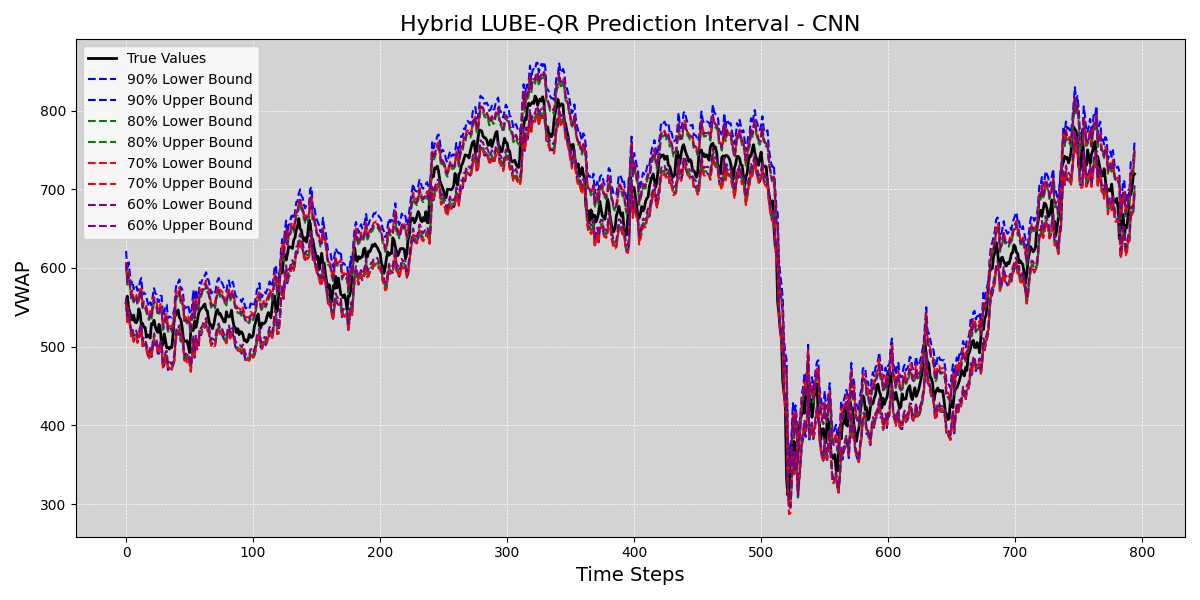
\includegraphics[width=\textwidth]{Chap03/figs/Hybrid_LUBE_QR_AllConfidence_axisbank_CNN.png}
            \caption{CNN.}
        \end{subfigure}
        \begin{subfigure}[b]{\textwidth}
            \centering
            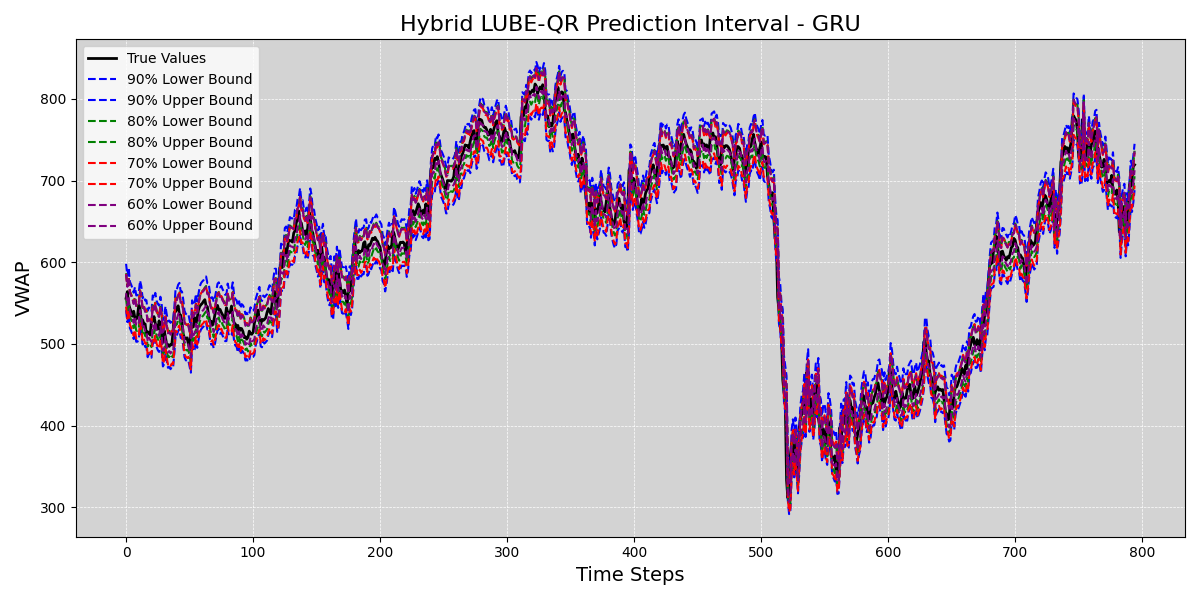
\includegraphics[width=\textwidth]{Chap03/figs/Hybrid_LUBE_QR_AllConfidence_axisbank_GRU.png}
            \caption{GRU.}
        \end{subfigure}
        \begin{subfigure}[b]{\textwidth}
            \centering
            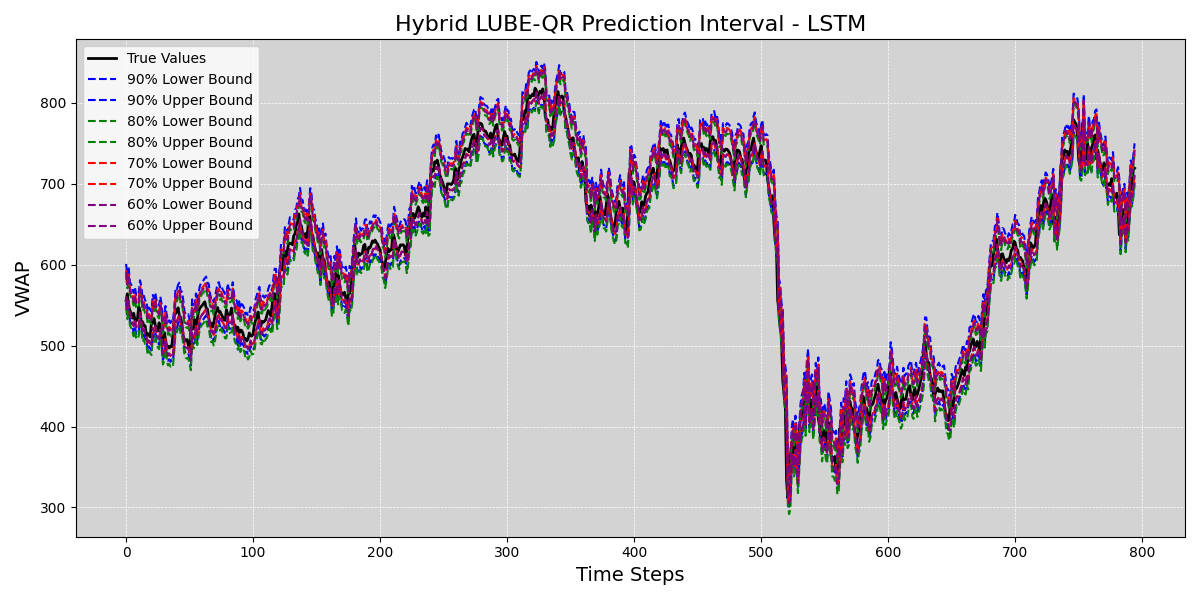
\includegraphics[width=\textwidth]{Chap03/figs/Hybrid_LUBE_QR_AllConfidence_axisbank_LSTM.png}
            \caption{LSTM.}
        \end{subfigure}
        \caption{Prediction Intervals for Axis Bank dataset obtained using proposed LUBE-QR based Hybrid Method and (a) BiLSTM, (b) CNN, (c) GRU, (d) LSTM Models respectively.}
        \label{fig 5.3}
    \end{minipage}
    \hfill
    \begin{minipage}{0.49\textwidth}
        \centering
        \begin{subfigure}[b]{\textwidth}
            \centering
            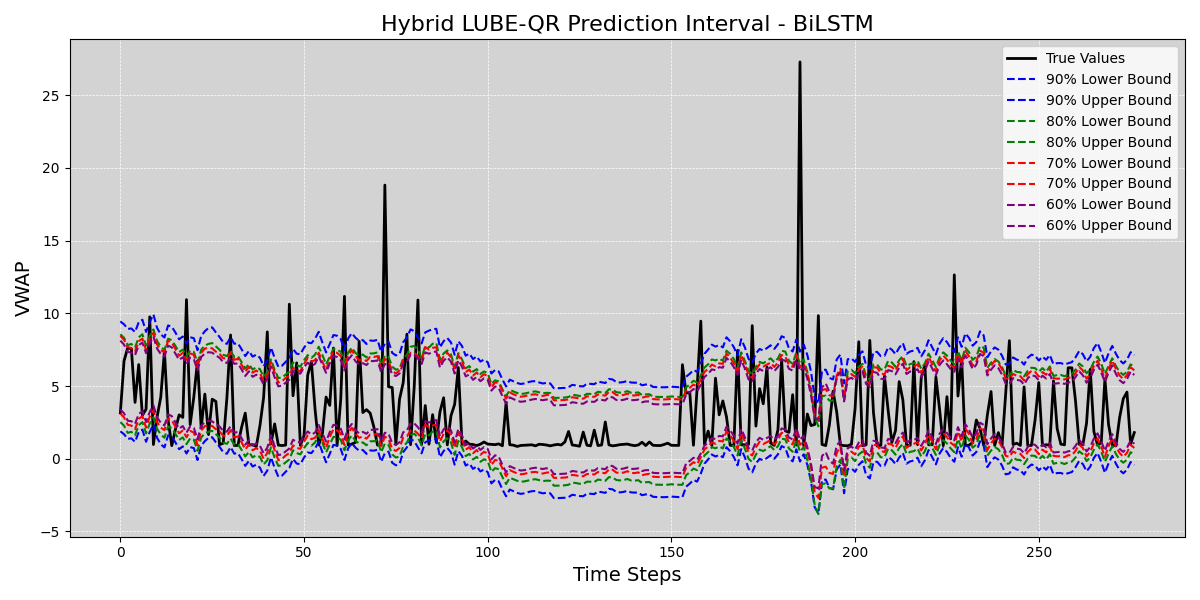
\includegraphics[width=\textwidth]{Chap03/figs/Hybrid_LUBE_QR_AllConfidence_elec_consumption_BiLSTM.png}
            \caption{BiLSTM.}
        \end{subfigure}
        \hfill
        \begin{subfigure}[b]{\textwidth}
            \centering
            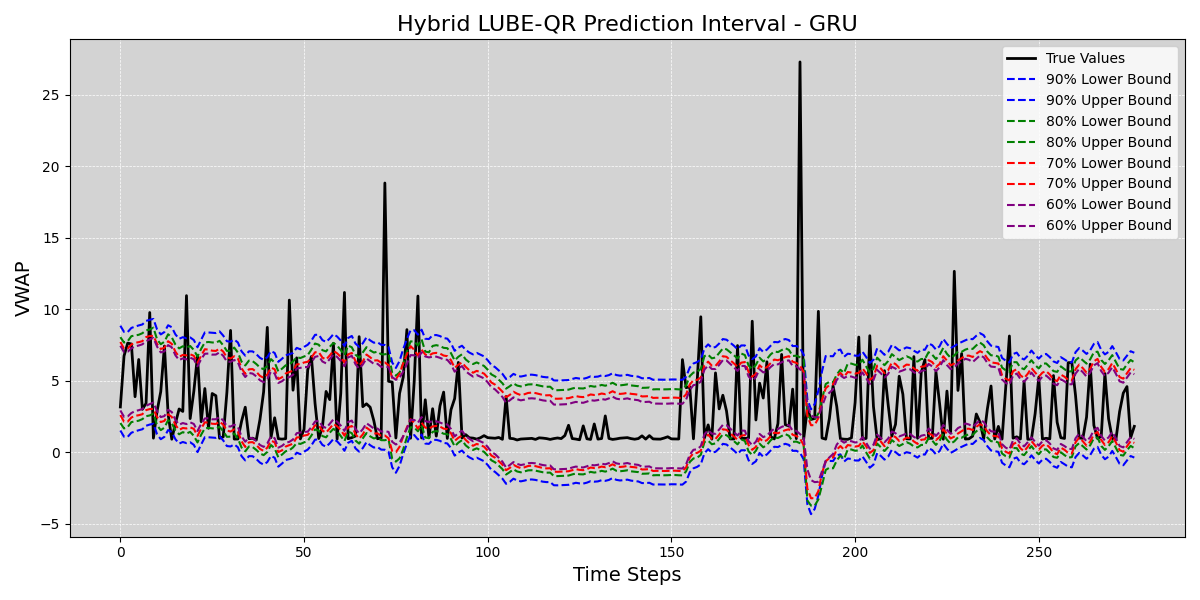
\includegraphics[width=\textwidth]{Chap03/figs/Hybrid_LUBE_QR_AllConfidence_elec_consumption_GRU.png}
            \caption{CNN.}
        \end{subfigure}
        \begin{subfigure}[b]{\textwidth}
            \centering
            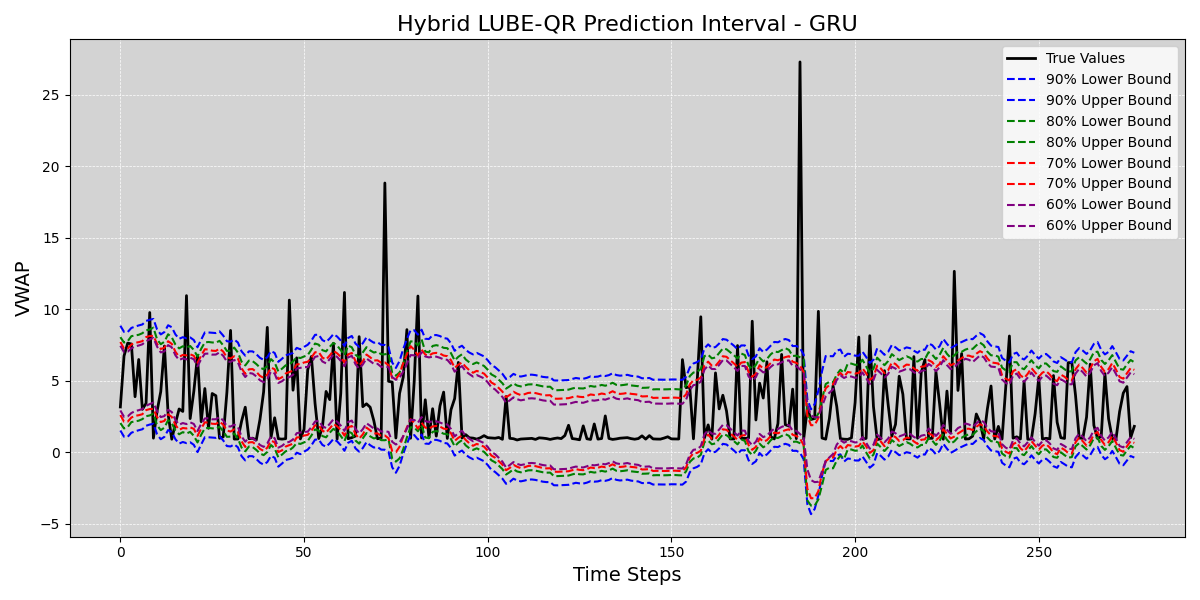
\includegraphics[width=\textwidth]{Chap03/figs/Hybrid_LUBE_QR_AllConfidence_elec_consumption_GRU.png}
            \caption{GRU.}
        \end{subfigure}
        \begin{subfigure}[b]{\textwidth}
            \centering
            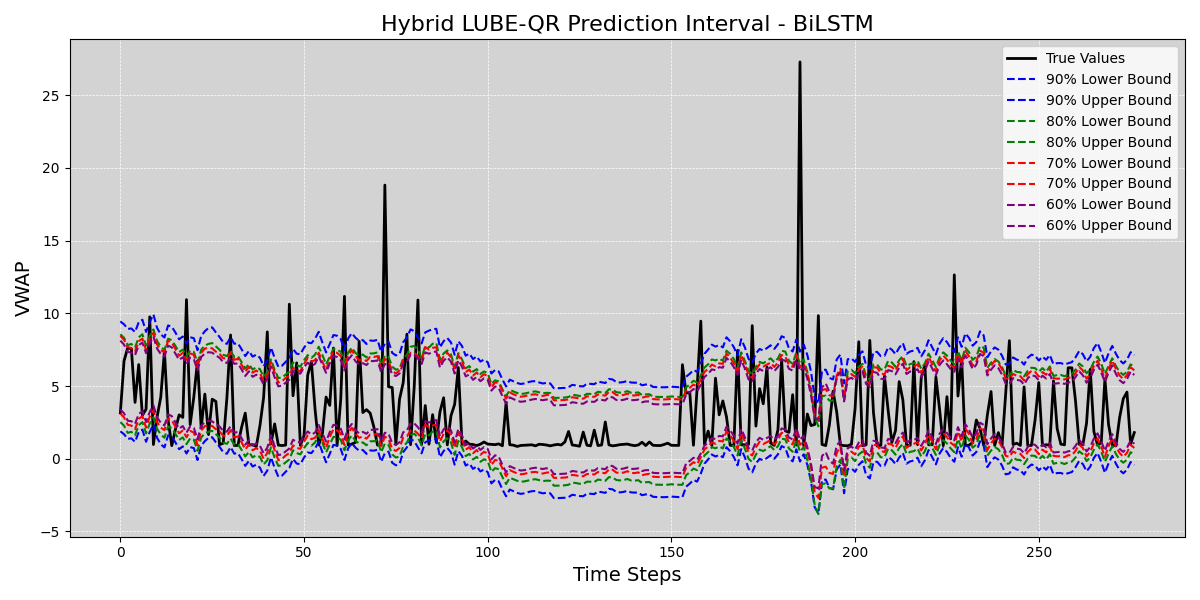
\includegraphics[width=\textwidth]{Chap03/figs/Hybrid_LUBE_QR_AllConfidence_elec_consumption_BiLSTM.png}
            \caption{LSTM.}
        \end{subfigure}
        \caption{Prediction Intervals for Electricity Consumption dataset obtained using proposed LUBE-QR based Hybrid Method and (a) BiLSTM, (b) CNN, (c) GRU, (d) LSTM Models respectively.}
        \label{fig 5.4}
    \end{minipage}
\end{figure}

\begin{figure}[H]
    \centering
        \begin{minipage}{0.50\textwidth}
            \centering
            \begin{subfigure}[b]{\textwidth}
                \centering
                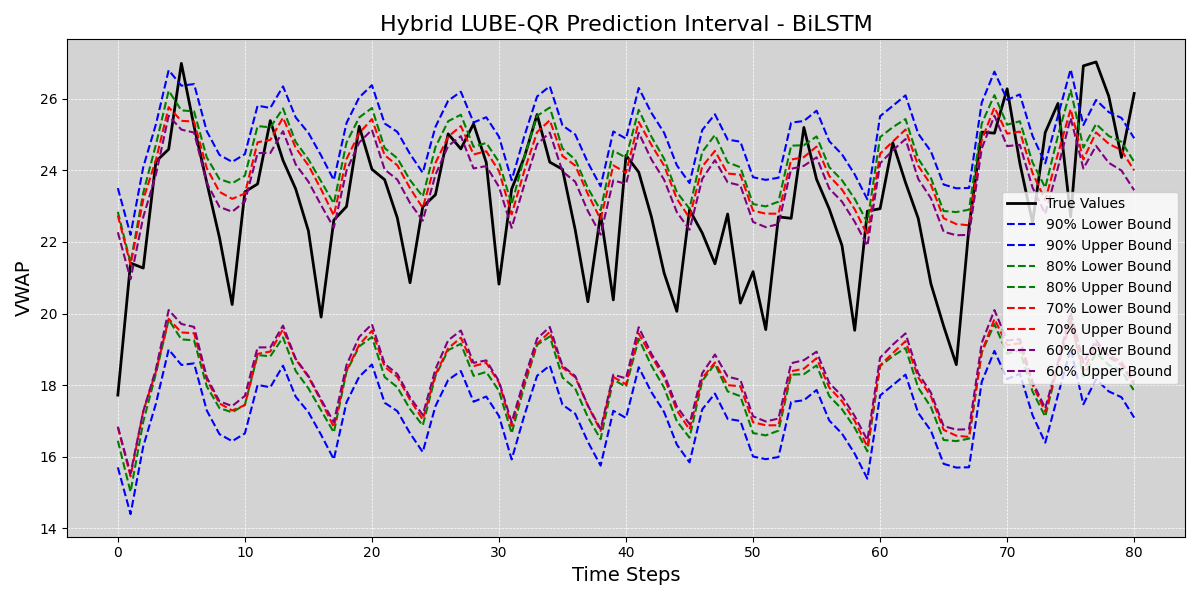
\includegraphics[width=\textwidth]{Chap03/figs/Hybrid_LUBE_QR_AllConfidence_web_traffic_BiLSTM.png}
                \caption{BiLSTM.}
            \end{subfigure}
            \hfill
            \begin{subfigure}[b]{\textwidth}
                \centering
                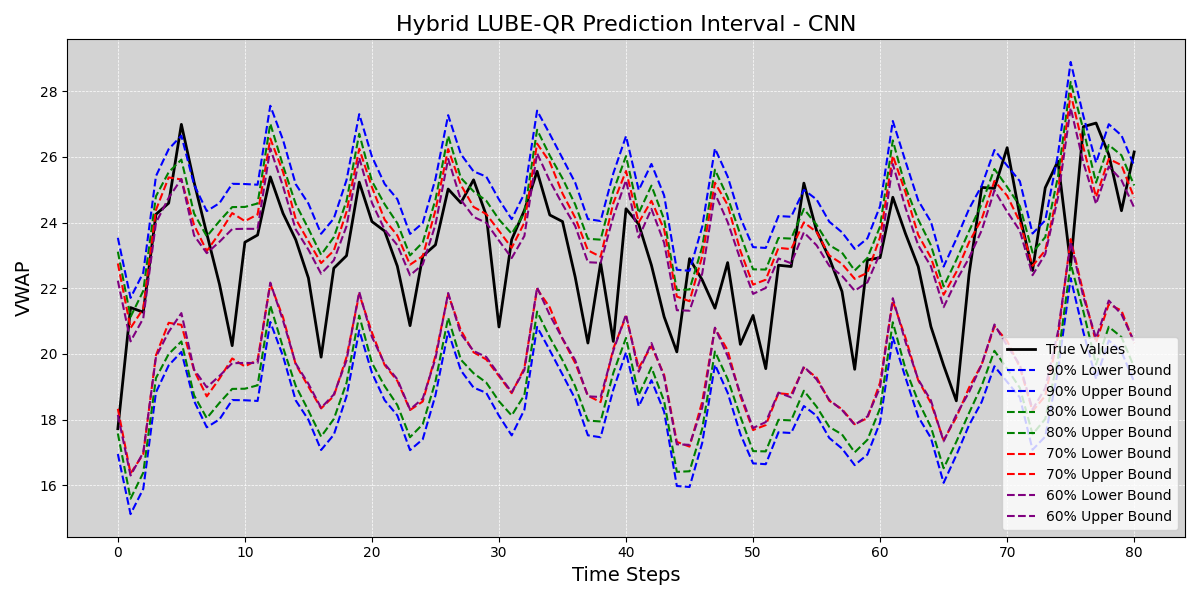
\includegraphics[width=\textwidth]{Chap03/figs/Hybrid_LUBE_QR_AllConfidence_web_traffic_CNN.png}
                \caption{CNN.}
            \end{subfigure}
            \begin{subfigure}[b]{\textwidth}
                \centering
                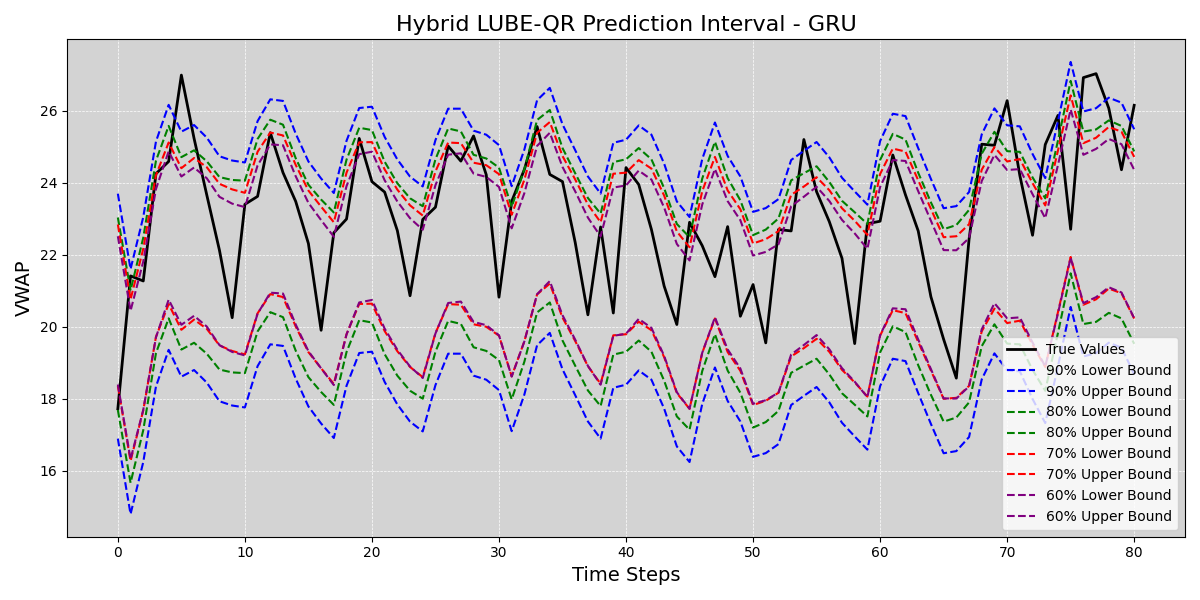
\includegraphics[width=\textwidth]{Chap03/figs/Hybrid_LUBE_QR_AllConfidence_web_traffic_GRU.png}
                \caption{GRU.}
            \end{subfigure}
            \begin{subfigure}[b]{\textwidth}
                \centering
                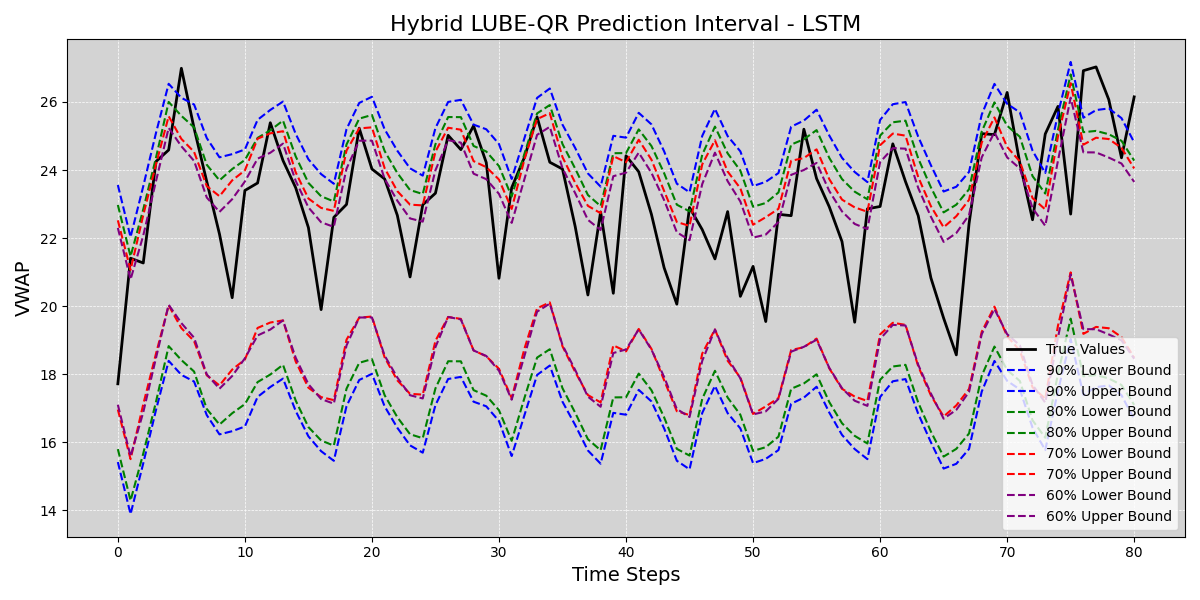
\includegraphics[width=\textwidth]{Chap03/figs/Hybrid_LUBE_QR_AllConfidence_web_traffic_LSTM.png}
                \caption{LSTM.}
            \end{subfigure}
        \end{minipage}
    
    \caption{Prediction Intervals for Web Traffic Load dataset obtained using proposed LUBE-QR based Hybrid Method and (a) BiLSTM, (b) CNN, (c) GRU, (d) LSTM Models respectively.}
    \label{fig 5.5}
\end{figure}
\clearpage

\begin{table*}[!t]
%\centering
\caption{Performance of LUBE-QR Hybrid Method on Adani Ports dataset.}
\vspace{0.5cm}
\renewcommand{\arraystretch}{1} % Adjust the value as needed
\resizebox{\textwidth}{!}{%
\begin{tabular}{|l|l|l|l|l|l|l|}
\hline
\textbf{Method Used} & \textbf{Confidence Level} & \textbf{Model} & \textbf{Avg PICP} & \textbf{Avg PINAW} &  \textbf{Avg ACE} & \textbf{Avg AWE} \\ \hline
\multirow{LUBE-QR Hybrid Method} 
& 0.6 & BiLSTM & 59.96 & 0.02 & 0.04 & 608.92  \\ \cline{2-7}
& 0.6 & CNN & 59.96 & 0.04 & 0.04 & 600.10 \\ \cline{2-7}
& 0.6 & GRU & 59.96 & 0.03 & 0.04 & 604.20 \\ \cline{2-7}
& 0.6 & LSTM & 59.96 & 0.02 & 0.04 & 608.53 \\ \cline{2-7}
& 0.7 & BiLSTM & 70.02 & 0.03 & 0.02 & 602.85 \\ \cline{2-7}
& 0.7 & CNN & 70.02 & 0.04 & 0.02 & 600.50 \\  \cline{2-7}
& 0.7 & GRU & 70.02 & 0.03 & 0.02 & 602.87 \\ \cline{2-7}
& 0.7 & LSTM & 70.02 & 0.03 & 0.02 & 602.49 \\ \cline{2-7}
& 0.8 & BiLSTM & 79.88 & 0.04 & 0.12 & 599.96 \\ \cline{2-7}
& 0.8 & CNN & 79.88 & 0.05 & 0.12 & 590.15 \\ \cline{2-7}
& 0.8 & GRU & 79.88 & 0.04 & 0.12 & 600.54 \\ \cline{2-7}
& 0.8 & LSTM & 79.88 & 0.05 & 0.12 & 593.65 \\ \cline{2-7}
& 0.9 & BiLSTM & 89.94 & 0.05 & 0.06 & 591.02 \\ \cline{2-7}
& 0.9 & CNN & 89.94 & 0.08 & 0.06 & 572.53 \\ \cline{2-7}
& 0.9 & GRU & 89.94 & 0.05 & 0.06 & 590.39 \\ \cline{2-7}
& 0.9 & LSTM & 89.94 & 0.06 & 0.06 & 583.94 \\ \hline
\end{tabular}%
}
\label{table 5.1}
\end{table*}

\begin{table*}[!t]
%\centering
\caption{Performance of LUBE-QR Hybrid Method on Asian Paints dataset.}
\vspace{0.5cm}
\renewcommand{\arraystretch}{1} % Adjust the value as needed
\resizebox{\textwidth}{!}{%
\begin{tabular}{|l|l|l|l|l|l|l|}
\hline
\textbf{Method Used} & \textbf{Confidence Level} & \textbf{Model} & \textbf{Avg PICP} & \textbf{Avg PINAW} &  \textbf{Avg ACE} & \textbf{Avg AWE} \\ \hline
\multirow{LUBE-QR Hybrid Method} 
& 0.6 & BiLSTM & 60.00 & 0.04 & 0.00 & 1679.25 \\ \cline{2-7}
& 0.6 & CNN & 60.00 & 0.05 & 0.00 & 1660.44 \\ \cline{2-7}
& 0.6 & GRU & 60.00 & 0.02 & 0.00 & 1704.50 \\ \cline{2-7}
& 0.6 & LSTM & 60.00 & 0.06 & 0.00 & 1639.36 \\ \cline{2-7}
& 0.7 & BiLSTM & 69.94 & 0.03 & 0.06 & 1687.10 \\ \cline{2-7}
& 0.7 & CNN & 69.94 & 0.04 & 0.06 & 1668.43 \\ \cline{2-7}
& 0.7 & GRU & 69.94 & 0.04 & 0.06 & 1675.49 \\ \cline{2-7}
& 0.7 & LSTM & 69.94 & 0.04 & 0.06 & 1670.81 \\ \cline{2-7}
& 0.8 & BiLSTM & 80.00 & 0.04 & 0.00 & 1679.75 \\ \cline{2-7}
& 0.8 & CNN & 80.00 & 0.05 & 0.00 & 1659.36 \\ \cline{2-7}
& 0.8 & GRU & 80.00 & 0.04 & 0.00 & 1685.31 \\ \cline{2-7}
& 0.8 & LSTM & 80.00 & 0.05 & 0.00 & 1662.02 \\ \cline{2-7}
& 0.9 & BiLSTM & 89.94 & 0.08 & 0.06 & 1603.47 \\ \cline{2-7}
& 0.9 & CNN & 89.94 & 0.08 & 0.06 & 1608.31 \\ \cline{2-7}
& 0.9 & GRU & 89.94 & 0.06 & 0.06 & 1637.27 \\ \cline{2-7}
& 0.9 & LSTM & 89.94 & 0.07 & 0.06 & 1620.58 \\ \hline

\end{tabular}%
}
\label{table 5.2}
\end{table*}

\clearpage

\begin{table*}[!t]
%\centering
\caption{Performance of LUBE-QR Hybrid Method on Axis Bank dataset.}
\vspace{0.5cm}
\renewcommand{\arraystretch}{1} % Adjust the value as needed
\resizebox{\textwidth}{!}{%
\begin{tabular}{|l|l|l|l|l|l|l|}
\hline
\textbf{Method Used} & \textbf{Confidence Level} & \textbf{Model} & \textbf{Avg PICP} & \textbf{Avg PINAW} &  \textbf{Avg ACE} & \textbf{Avg AWE} \\ \hline
\multirow{LUBE-QR Hybrid Method} 
& 0.6 & BiLSTM & 60.00 & 0.05 & 0.00 & 482.85 \\ \cline{2-7}
& 0.6 & CNN & 60.00 & 0.09 & 0.00 & 463.85 \\ \cline{2-7}
& 0.6 & GRU & 60.00 & 0.05 & 0.00 & 483.88 \\ \cline{2-7}
& 0.6 & LSTM & 60.00 & 0.06 & 0.00 & 476.72 \\ \cline{2-7}
& 0.7 & BiLSTM & 69.94 & 0.05 & 0.06 & 482.26 \\ \cline{2-7}
& 0.7 & CNN & 69.94 & 0.11 & 0.06 & 452.96 \\ \cline{2-7}
& 0.7 & GRU & 69.94 & 0.08 & 0.06 & 466.92 \\ \cline{2-7}
& 0.7 & LSTM & 69.94 & 0.06 & 0.06 & 474.35 \\ \cline{2-7}
& 0.8 & BiLSTM & 80.00 & 0.06 & 0.00 & 477.10 \\ \cline{2-7}
& 0.8 & CNN & 80.00 & 0.09 & 0.00 & 462.02 \\ \cline{2-7}
& 0.8 & GRU & 80.00 & 0.06 & 0.00 & 475.72 \\ \cline{2-7}
& 0.8 & LSTM & 80.00 & 0.07 & 0.00 & 468.94 \\ \cline{2-7}
& 0.9 & BiLSTM & 89.94 & 0.08 & 0.06 & 467.31 \\ \cline{2-7}
& 0.9 & CNN & 89.94 & 0.13 & 0.06 & 441.30 \\ \cline{2-7}
& 0.9 & GRU & 89.94 & 0.11 & 0.06 & 450.19 \\ \cline{2-7}
& 0.9 & LSTM & 89.94 & 0.09 & 0.06 & 458.83 \\ \hline

\end{tabular}%
}
\label{table 5.3}
\end{table*}


\begin{table*}[!t]
%\centering
\caption{Performance of LUBE-QR Hybrid Method on Electricity Consumption dataset.}
\vspace{0.5cm}
\renewcommand{\arraystretch}{1} % Adjust the value as needed
\resizebox{\textwidth}{!}{%
\begin{tabular}{|l|l|l|l|l|l|l|}
\hline
\textbf{Method Used} & \textbf{Confidence Level} & \textbf{Model} & \textbf{Avg PICP} & \textbf{Avg PINAW} &  \textbf{Avg ACE} & \textbf{Avg AWE} \\ \hline
\multirow{LUBE-QR Hybrid Method} 
& 0.6 & BiLSTM & 59.93 & 0.18 & 0.07 & 21.71 \\ \cline{2-7}
& 0.6 & CNN & 59.93 & 0.17 & 0.07 & 22.00 \\ \cline{2-7}
& 0.6 & GRU & 59.93 & 0.17 & 0.07 & 21.92 \\ \cline{2-7}
& 0.6 & LSTM & 59.93 & 0.16 & 0.07 & 22.10 \\ \cline{2-7}
& 0.7 & BiLSTM & 70.04 & 0.20 & 0.04 & 21.11 \\ \cline{2-7}
& 0.7 & CNN & 70.04 & 0.21 & 0.04 & 20.96 \\ \cline{2-7}
& 0.7 & GRU & 70.04 & 0.19 & 0.04 & 21.33 \\ \cline{2-7}
& 0.7 & LSTM & 70.04 & 0.19 & 0.04 & 21.51 \\ \cline{2-7}
& 0.8 & BiLSTM & 79.78 & 0.23 & 0.22 & 20.40 \\ \cline{2-7}
& 0.8 & CNN & 79.78 & 0.25 & 0.22 & 19.89 \\ \cline{2-7}
& 0.8 & GRU & 79.78 & 0.23 & 0.22 & 20.43 \\ \cline{2-7}
& 0.8 & LSTM & 79.78 & 0.22 & 0.22 & 20.61 \\ \cline{2-7}
& 0.9 & BiLSTM & 89.89 & 0.29 & 0.11 & 18.88 \\ \cline{2-7}
& 0.9 & CNN & 89.89 & 0.32 & 0.11 & 17.87 \\ \cline{2-7}
& 0.9 & GRU & 89.89 & 0.28 & 0.11 & 19.11 \\ \cline{2-7}
& 0.9 & LSTM & 89.89 & 0.29 & 0.11 & 18.90 \\ \hline
\end{tabular}%
}
\label{table 5.4}
\end{table*}

\clearpage
\begin{table*}[!t]
%\centering
\caption{Performance of LUBE-QR Hybrid Method on Web Traffic dataset.}
\vspace{0.5cm}
\renewcommand{\arraystretch}{1} % Adjust the value as needed
\resizebox{\textwidth}{!}{%
\begin{tabular}{|l|l|l|l|l|l|l|}
\hline
\textbf{Method Used} & \textbf{Confidence Level} & \textbf{Model} & \textbf{Avg PICP} & \textbf{Avg PINAW} &  \textbf{Avg ACE} & \textbf{Avg AWE} \\ \hline
\multirow{LUBE-QR Hybrid Method} 
& 0.6 & BiLSTM & 60.25 & 0.58 & 0.54 & 3.88 \\ \cline{2-7}
& 0.6 & CNN & 60.00 & 0.44 & 0.59 & 5.23 \\ \cline{2-7}
& 0.6 & GRU & 60.37 & 0.44 & 0.52 & 5.19 \\ \cline{2-7}
& 0.6 & LSTM & 60.49 & 0.56 & 0.49 & 4.12 \\ \cline{2-7}
& 0.7 & BiLSTM & 69.75 & 0.64 & 0.62 & 3.40 \\ \cline{2-7}
& 0.7 & CNN & 69.63 & 0.48 & 0.67 & 4.88 \\ \cline{2-7}
& 0.7 & GRU & 70.00 & 0.48 & 0.52 & 4.82 \\ \cline{2-7}
& 0.7 & LSTM & 69.75 & 0.60 & 0.62 & 3.75 \\ \cline{2-7}
& 0.8 & BiLSTM & 79.14 & 0.69 & 0.91 & 2.91 \\ \cline{2-7}
& 0.8 & CNN & 79.38 & 0.59 & 0.77 & 3.77 \\ \cline{2-7}
& 0.8 & GRU & 79.75 & 0.57 & 0.54 & 3.96 \\ \cline{2-7}
& 0.8 & LSTM & 79.26 & 0.77 & 0.84 & 2.35 \\ \cline{2-7}
& 0.9 & BiLSTM & 89.01 & 0.84 & 1.01 & 1.51 \\ \cline{2-7}
& 0.9 & CNN & 89.14 & 0.71 & 0.91 & 2.72 \\ \cline{2-7}
& 0.9 & GRU & 89.01 & 0.73 & 1.01 & 2.50 \\ \cline{2-7}
& 0.9 & LSTM & 89.38 & 0.87 & 0.72 & 1.39 \\ \hline

\end{tabular}%
}
\label{table 5.5}
\end{table*}
%\clearpage

\subsection{Statistical Analysis}
Figures \ref{fig 4.6} and \ref{fig 4.7} shows the Friedman-Nemenyi hypothesis results obtained on the PINAW and ACE Metrics respectively across all the five datasets and all the eight different methods (Each method is coupled with a Deep Learning Model with which it had performed best). It proves that the proposed LUBE-QR based Hybrid Method is a statistically better or equivalent method to other existing Traditional Probabilistic Forecasting methods.
%\clearpage
\begin{figure}
    \centering
    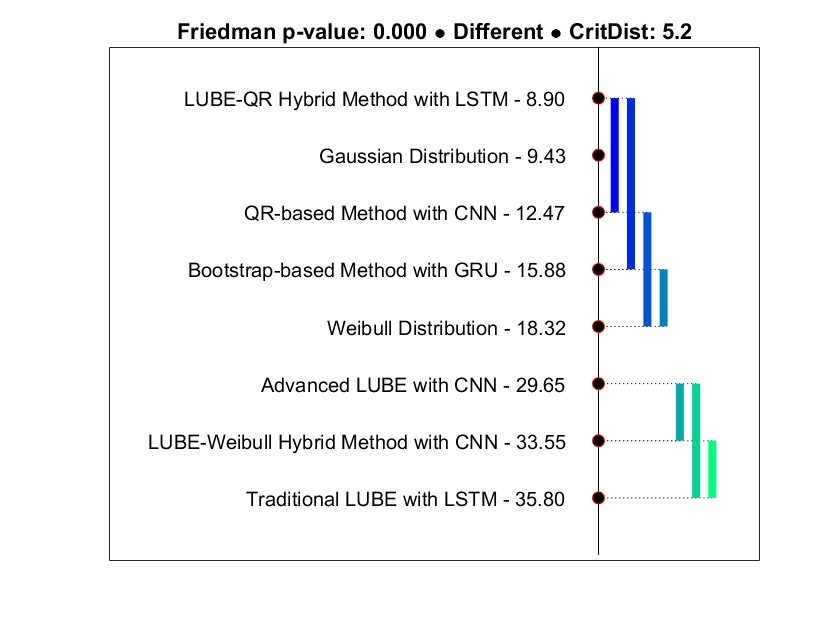
\includegraphics[width=0.6\linewidth]{Chap03/figs/Statistical_Analysis_All_Methods_PINAW.jpg}
    \caption{Statistical Analysis on PINAW Metric performed on all the five datasets together.}
    \label{fig 4.6}
\end{figure}
\clearpage
\begin{figure}
    \centering
    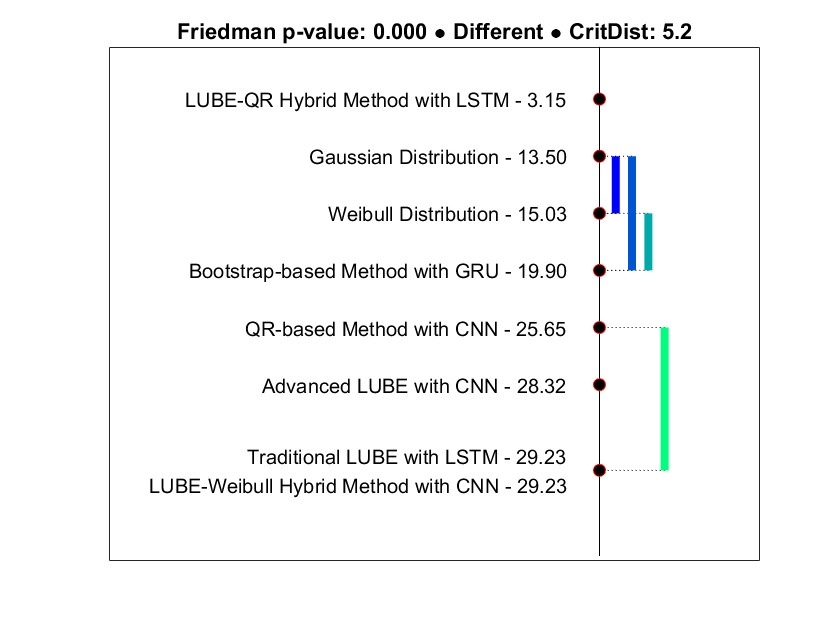
\includegraphics[width=0.6\linewidth]{Chap03/figs/Statistical_Analysis_All_Methods_ACE.jpg}
    \caption{Statistical Analysis on ACE Metric performed on all the five datasets together.}
    \label{fig 4.7}
\end{figure}

\subsection{Discussion}
The hybrid method based on LUBE–QR that has been proposed introduces a new solution for increasing the reliability and sharpness of prediction intervals for probabilistic time series forecasting. By capitalizing on the respective strengths of both the Advanced LUBE technique and Quantile Regression (QR), the approach is able to overcome the limitations within each individual technique. The LUBE component achieves direct interval prediction using deep learning with self-defined loss optimization, and QR supplies data-driven correction of residual errors to enhance the adaptiveness of predicted bounds.

Experimental results show that the hybrid approach persistently yields smaller ACE (Absolute Coverage Error) and PINAW (Prediction Interval Normalized Average Width) values than individual LUBE, QR, or other baseline models on several deep learning architectures (LSTM, BiLSTM, CNN, GRU). This shows that the hybrid intervals are both narrow and well-calibrated, the best combination for good uncertainty quantification. The Friedman–Nemenyi hypothesis test also verifies the statistical performance superiority of the hybrid method, with the method being ranked first with all evaluation metrics in various confidence levels (0.6 to 0.9).

In general, the hybridization of LUBE and QR is a strong and effective approach to generating high-quality prediction intervals and one that can chart a promising path forward for uncertainty-aware forecasting in the future.

\section{Summary}
In this chapter, we proposed a novel LUBE–QR hybrid technique that seamlessly blends the interval forecasting capabilities of the Advanced LUBE method with quantile regression on residuals' flexibility. By joining these two approaches, the proposed method provided more precise and sharper prediction intervals at different levels of confidence as verified through detailed experiments and evaluation metrics. In contrast to traditional approaches which tend to have a compromise between interval width and coverage, the hybrid approach presents a better balanced trade-off. The uniformity of performance in various deep learning models and statistical superiority as witnessed by the Friedman–Nemenyi test reflect its strength. 
In the future, follow-up work may investigate extending this hybrid model to multivariate time series forecasting and real-time adaptive interval updates and incorporating sophisticated ensemble methods or probabilistic Bayesian layers to further boost uncertainty quantification in dynamic high-noise conditions.


\chapter{Conclusion and Future Work}

In this thesis we have first conducted a thorough study of Traditional Probabilistic Forecasting methods divided into two groups: Parametric under which we've covered Gaussian Distribution based Method and Weibull Distribution based Method and Non-parametric under which we've covered Traditional LUBE, Advanced LUBE, QR-based Method and Bootstrap-based Method. We have evaluated the non-parametric methods using four different Deep Learning Models: LSTM, CNN, GRU and BiLSTM across four different confidence levels 90\%, 80\%, 70\% and 60\% and also run simulations for ten times to obtain the average results and then plotted the graphs using the obtained results. We have then compared the results to conclude the best performing Traditional Probabilistic Forecasting Method.

Then, we developed our first Hybrid method using two different existing methods Traditional LUBE Method and Weibull Distribution based Method. We used the same four DL models to assess it's performance across the four different confidence levels and obtained average results and graphs in a similar fashion. The key takeaway from this Hybrid Method was that it performed close to Advacned LUBE method giving similar PICP values (close to 100, thus making the intervals wide and reducing sharpness) while being computationally very efficient and thus it can effectively replace systems using Traditionl LUBE, Advanced LUBE or other computationally heavy methods with a slight tradeoff for wider intervals (conservative performance).

Next, we developed our second Hybrid method using two different and popular Non-Parametric based methods namely Advanced LUBE and QR-based Methods. This method achieved the best results that we've gotten so far from any model. It achieved PICP values closer to the actual confidence levels and maintained the lowest PINAW, ACE and AWE values. It produced crisp and sharp intervals while barely overfitting or underfitting the data. This method can be used as an effective alternative to existing traditional probabilistic forecasting methods but it can be a bit computationally intensive.

Future Work may include deep diving into more hybrid methods by combining and fusing multiple existing methods with various different DL models to achieve better probabilistic forecasting results.